\documentclass[twoside]{book}

% Packages required by doxygen
\usepackage{fixltx2e}
\usepackage{calc}
\usepackage{doxygen}
\usepackage[export]{adjustbox} % also loads graphicx
\usepackage{graphicx}
\usepackage[utf8]{inputenc}
\usepackage{makeidx}
\usepackage{multicol}
\usepackage{multirow}
\PassOptionsToPackage{warn}{textcomp}
\usepackage{textcomp}
\usepackage[nointegrals]{wasysym}
\usepackage[table]{xcolor}

% Font selection
\usepackage[T1]{fontenc}
\usepackage[scaled=.90]{helvet}
\usepackage{courier}
\usepackage{amssymb}
\usepackage{sectsty}
\renewcommand{\familydefault}{\sfdefault}
\allsectionsfont{%
  \fontseries{bc}\selectfont%
  \color{darkgray}%
}
\renewcommand{\DoxyLabelFont}{%
  \fontseries{bc}\selectfont%
  \color{darkgray}%
}
\newcommand{\+}{\discretionary{\mbox{\scriptsize$\hookleftarrow$}}{}{}}

% Page & text layout
\usepackage{geometry}
\geometry{%
  a4paper,%
  top=2.5cm,%
  bottom=2.5cm,%
  left=2.5cm,%
  right=2.5cm%
}
\tolerance=750
\hfuzz=15pt
\hbadness=750
\setlength{\emergencystretch}{15pt}
\setlength{\parindent}{0cm}
\setlength{\parskip}{3ex plus 2ex minus 2ex}
\makeatletter
\renewcommand{\paragraph}{%
  \@startsection{paragraph}{4}{0ex}{-1.0ex}{1.0ex}{%
    \normalfont\normalsize\bfseries\SS@parafont%
  }%
}
\renewcommand{\subparagraph}{%
  \@startsection{subparagraph}{5}{0ex}{-1.0ex}{1.0ex}{%
    \normalfont\normalsize\bfseries\SS@subparafont%
  }%
}
\makeatother

% Headers & footers
\usepackage{fancyhdr}
\pagestyle{fancyplain}
\fancyhead[LE]{\fancyplain{}{\bfseries\thepage}}
\fancyhead[CE]{\fancyplain{}{}}
\fancyhead[RE]{\fancyplain{}{\bfseries\leftmark}}
\fancyhead[LO]{\fancyplain{}{\bfseries\rightmark}}
\fancyhead[CO]{\fancyplain{}{}}
\fancyhead[RO]{\fancyplain{}{\bfseries\thepage}}
\fancyfoot[LE]{\fancyplain{}{}}
\fancyfoot[CE]{\fancyplain{}{}}
\fancyfoot[RE]{\fancyplain{}{\bfseries\scriptsize Generated by Doxygen }}
\fancyfoot[LO]{\fancyplain{}{\bfseries\scriptsize Generated by Doxygen }}
\fancyfoot[CO]{\fancyplain{}{}}
\fancyfoot[RO]{\fancyplain{}{}}
\renewcommand{\footrulewidth}{0.4pt}
\renewcommand{\chaptermark}[1]{%
  \markboth{#1}{}%
}
\renewcommand{\sectionmark}[1]{%
  \markright{\thesection\ #1}%
}

% Indices & bibliography
\usepackage{natbib}
\usepackage[titles]{tocloft}
\setcounter{tocdepth}{3}
\setcounter{secnumdepth}{5}
\makeindex

% Hyperlinks (required, but should be loaded last)
\usepackage{ifpdf}
\ifpdf
  \usepackage[pdftex,pagebackref=true]{hyperref}
\else
  \usepackage[ps2pdf,pagebackref=true]{hyperref}
\fi
\hypersetup{%
  colorlinks=true,%
  linkcolor=blue,%
  citecolor=blue,%
  unicode%
}

% Custom commands
\newcommand{\clearemptydoublepage}{%
  \newpage{\pagestyle{empty}\cleardoublepage}%
}

\usepackage{caption}
\captionsetup{labelsep=space,justification=centering,font={bf},singlelinecheck=off,skip=4pt,position=top}

%===== C O N T E N T S =====

\begin{document}

% Titlepage & ToC
\hypersetup{pageanchor=false,
             bookmarksnumbered=true,
             pdfencoding=unicode
            }
\pagenumbering{alph}
\begin{titlepage}
\vspace*{7cm}
\begin{center}%
{\Large pmp }\\
\vspace*{1cm}
{\large Generated by Doxygen 1.8.13}\\
\end{center}
\end{titlepage}
\clearemptydoublepage
\pagenumbering{roman}
\tableofcontents
\clearemptydoublepage
\pagenumbering{arabic}
\hypersetup{pageanchor=true}

%--- Begin generated contents ---
\chapter{Namespace Index}
\section{Namespace List}
Here is a list of all namespaces with brief descriptions\+:\begin{DoxyCompactList}
\item\contentsline{section}{\hyperlink{namespaceLogger}{Logger} }{\pageref{namespaceLogger}}{}
\item\contentsline{section}{\hyperlink{namespaceMandelbrot}{Mandelbrot} }{\pageref{namespaceMandelbrot}}{}
\item\contentsline{section}{\hyperlink{namespacePGM}{P\+GM} }{\pageref{namespacePGM}}{}
\item\contentsline{section}{\hyperlink{namespaceProtocol}{Protocol} }{\pageref{namespaceProtocol}}{}
\item\contentsline{section}{\hyperlink{namespaceTcpBackend}{Tcp\+Backend} }{\pageref{namespaceTcpBackend}}{}
\end{DoxyCompactList}

\chapter{Hierarchical Index}
\section{Class Hierarchy}
This inheritance list is sorted roughly, but not completely, alphabetically\+:\begin{DoxyCompactList}
\item \contentsline{section}{Tcp\+Backend\+:\+:Client}{\pageref{classTcpBackend_1_1Client}}{}
\begin{DoxyCompactList}
\item \contentsline{section}{Tcp\+Backend\+:\+:Client\+Asio}{\pageref{classTcpBackend_1_1ClientAsio}}{}
\end{DoxyCompactList}
\item \contentsline{section}{Tcp\+Backend\+:\+:Connection}{\pageref{classTcpBackend_1_1Connection}}{}
\begin{DoxyCompactList}
\item \contentsline{section}{Tcp\+Backend\+:\+:Connection\+Asio}{\pageref{classTcpBackend_1_1ConnectionAsio}}{}
\end{DoxyCompactList}
\item \contentsline{section}{Protocol\+:\+:Request}{\pageref{structProtocol_1_1Request}}{}
\item \contentsline{section}{Protocol\+:\+:Response}{\pageref{structProtocol_1_1Response}}{}
\item \contentsline{section}{Tcp\+Backend\+:\+:Server}{\pageref{classTcpBackend_1_1Server}}{}
\begin{DoxyCompactList}
\item \contentsline{section}{Tcp\+Backend\+:\+:Server\+Asio}{\pageref{classTcpBackend_1_1ServerAsio}}{}
\end{DoxyCompactList}
\item \contentsline{section}{Session}{\pageref{structSession}}{}
\item Tcp\+Connection\begin{DoxyCompactList}
\item \contentsline{section}{Tcp\+Connection\+Epoll}{\pageref{classTcpConnectionEpoll}}{}
\end{DoxyCompactList}
\item Tcp\+Server\begin{DoxyCompactList}
\item \contentsline{section}{Tcp\+Server\+Epoll}{\pageref{classTcpServerEpoll}}{}
\end{DoxyCompactList}
\end{DoxyCompactList}

\chapter{Data Structure Index}
\section{Data Structures}
Here are the data structures with brief descriptions\+:\begin{DoxyCompactList}
\item\contentsline{section}{\hyperlink{classTcpBackend_1_1Client}{Tcp\+Backend\+::\+Client} \\*Used to start a connection }{\pageref{classTcpBackend_1_1Client}}{}
\item\contentsline{section}{\hyperlink{classTcpBackend_1_1ClientAsio}{Tcp\+Backend\+::\+Client\+Asio} }{\pageref{classTcpBackend_1_1ClientAsio}}{}
\item\contentsline{section}{\hyperlink{classTcpBackend_1_1Connection}{Tcp\+Backend\+::\+Connection} \\*Represents a connection }{\pageref{classTcpBackend_1_1Connection}}{}
\item\contentsline{section}{\hyperlink{classTcpBackend_1_1ConnectionAsio}{Tcp\+Backend\+::\+Connection\+Asio} }{\pageref{classTcpBackend_1_1ConnectionAsio}}{}
\item\contentsline{section}{\hyperlink{structProtocol_1_1Request}{Protocol\+::\+Request} }{\pageref{structProtocol_1_1Request}}{}
\item\contentsline{section}{\hyperlink{structProtocol_1_1Response}{Protocol\+::\+Response} }{\pageref{structProtocol_1_1Response}}{}
\item\contentsline{section}{\hyperlink{classTcpBackend_1_1Server}{Tcp\+Backend\+::\+Server} \\*Used to accept new connections }{\pageref{classTcpBackend_1_1Server}}{}
\item\contentsline{section}{\hyperlink{classTcpBackend_1_1ServerAsio}{Tcp\+Backend\+::\+Server\+Asio} }{\pageref{classTcpBackend_1_1ServerAsio}}{}
\item\contentsline{section}{\hyperlink{structSession}{Session} }{\pageref{structSession}}{}
\item\contentsline{section}{\hyperlink{classTcpConnectionEpoll}{Tcp\+Connection\+Epoll} }{\pageref{classTcpConnectionEpoll}}{}
\item\contentsline{section}{\hyperlink{classTcpServerEpoll}{Tcp\+Server\+Epoll} }{\pageref{classTcpServerEpoll}}{}
\end{DoxyCompactList}

\chapter{File Index}
\section{File List}
Here is a list of all files with brief descriptions\+:\begin{DoxyCompactList}
\item\contentsline{section}{src/\hyperlink{logger_8cc}{logger.\+cc} }{\pageref{logger_8cc}}{}
\item\contentsline{section}{src/\hyperlink{logger_8h}{logger.\+h} }{\pageref{logger_8h}}{}
\item\contentsline{section}{src/\hyperlink{mandelbrot_8cc}{mandelbrot.\+cc} }{\pageref{mandelbrot_8cc}}{}
\item\contentsline{section}{src/\hyperlink{mandelbrot_8h}{mandelbrot.\+h} }{\pageref{mandelbrot_8h}}{}
\item\contentsline{section}{src/\hyperlink{pgm_8cc}{pgm.\+cc} }{\pageref{pgm_8cc}}{}
\item\contentsline{section}{src/\hyperlink{pgm_8h}{pgm.\+h} }{\pageref{pgm_8h}}{}
\item\contentsline{section}{src/\hyperlink{pmp__client_8cc}{pmp\+\_\+client.\+cc} }{\pageref{pmp__client_8cc}}{}
\item\contentsline{section}{src/\hyperlink{pmp__server_8cc}{pmp\+\_\+server.\+cc} }{\pageref{pmp__server_8cc}}{}
\item\contentsline{section}{src/\hyperlink{protocol_8cc}{protocol.\+cc} }{\pageref{protocol_8cc}}{}
\item\contentsline{section}{src/\hyperlink{protocol_8h}{protocol.\+h} }{\pageref{protocol_8h}}{}
\item\contentsline{section}{src/\hyperlink{tcp__backend_8h}{tcp\+\_\+backend.\+h} }{\pageref{tcp__backend_8h}}{}
\item\contentsline{section}{src/backend\+\_\+asio/\hyperlink{tcp__backend__asio_8cc}{tcp\+\_\+backend\+\_\+asio.\+cc} }{\pageref{tcp__backend__asio_8cc}}{}
\item\contentsline{section}{src/backend\+\_\+asio/\hyperlink{tcp__client__asio_8cc}{tcp\+\_\+client\+\_\+asio.\+cc} }{\pageref{tcp__client__asio_8cc}}{}
\item\contentsline{section}{src/backend\+\_\+asio/\hyperlink{tcp__client__asio_8h}{tcp\+\_\+client\+\_\+asio.\+h} }{\pageref{tcp__client__asio_8h}}{}
\item\contentsline{section}{src/backend\+\_\+asio/\hyperlink{tcp__connection__asio_8cc}{tcp\+\_\+connection\+\_\+asio.\+cc} }{\pageref{tcp__connection__asio_8cc}}{}
\item\contentsline{section}{src/backend\+\_\+asio/\hyperlink{tcp__connection__asio_8h}{tcp\+\_\+connection\+\_\+asio.\+h} }{\pageref{tcp__connection__asio_8h}}{}
\item\contentsline{section}{src/backend\+\_\+asio/\hyperlink{tcp__server__asio_8cc}{tcp\+\_\+server\+\_\+asio.\+cc} }{\pageref{tcp__server__asio_8cc}}{}
\item\contentsline{section}{src/backend\+\_\+asio/\hyperlink{tcp__server__asio_8h}{tcp\+\_\+server\+\_\+asio.\+h} }{\pageref{tcp__server__asio_8h}}{}
\item\contentsline{section}{src/backend\+\_\+epoll/\hyperlink{tcp__connection__epoll_8cc}{tcp\+\_\+connection\+\_\+epoll.\+cc} }{\pageref{tcp__connection__epoll_8cc}}{}
\item\contentsline{section}{src/backend\+\_\+epoll/\hyperlink{tcp__connection__epoll_8h}{tcp\+\_\+connection\+\_\+epoll.\+h} }{\pageref{tcp__connection__epoll_8h}}{}
\item\contentsline{section}{src/backend\+\_\+epoll/\hyperlink{tcp__server__epoll_8cc}{tcp\+\_\+server\+\_\+epoll.\+cc} }{\pageref{tcp__server__epoll_8cc}}{}
\item\contentsline{section}{src/backend\+\_\+epoll/\hyperlink{tcp__server__epoll_8h}{tcp\+\_\+server\+\_\+epoll.\+h} }{\pageref{tcp__server__epoll_8h}}{}
\end{DoxyCompactList}

\chapter{Namespace Documentation}
\hypertarget{namespaceLogger}{}\section{Logger Namespace Reference}
\label{namespaceLogger}\index{Logger@{Logger}}
\subsection*{Enumerations}
\begin{DoxyCompactItemize}
\item 
enum \hyperlink{namespaceLogger_ad766a24576ea8b27ad9d5649cef46d8f}{Level} \{ \hyperlink{namespaceLogger_ad766a24576ea8b27ad9d5649cef46d8fa551b723eafd6a31d444fcb2f5920fbd3}{Level\+::\+I\+N\+FO}, 
\hyperlink{namespaceLogger_ad766a24576ea8b27ad9d5649cef46d8fadc30ec20708ef7b0f641ef78b7880a15}{Level\+::\+D\+E\+B\+UG}, 
\hyperlink{namespaceLogger_ad766a24576ea8b27ad9d5649cef46d8fabb1ca97ec761fc37101737ba0aa2e7c5}{Level\+::\+E\+R\+R\+OR}
 \}
\end{DoxyCompactItemize}
\subsection*{Functions}
\begin{DoxyCompactItemize}
\item 
void \hyperlink{namespaceLogger_a188a368bf6e884b7eba1236c39130364}{log} (const char $\ast$filename, int line, \hyperlink{namespaceLogger_ad766a24576ea8b27ad9d5649cef46d8f}{Level} level,...)
\end{DoxyCompactItemize}


\subsection{Enumeration Type Documentation}
\mbox{\Hypertarget{namespaceLogger_ad766a24576ea8b27ad9d5649cef46d8f}\label{namespaceLogger_ad766a24576ea8b27ad9d5649cef46d8f}} 
\index{Logger@{Logger}!Level@{Level}}
\index{Level@{Level}!Logger@{Logger}}
\subsubsection{\texorpdfstring{Level}{Level}}
{\footnotesize\ttfamily enum \hyperlink{namespaceLogger_ad766a24576ea8b27ad9d5649cef46d8f}{Logger\+::\+Level}\hspace{0.3cm}{\ttfamily [strong]}}

\begin{DoxyEnumFields}{Enumerator}
\raisebox{\heightof{T}}[0pt][0pt]{\index{I\+N\+FO@{I\+N\+FO}!Logger@{Logger}}\index{Logger@{Logger}!I\+N\+FO@{I\+N\+FO}}}\mbox{\Hypertarget{namespaceLogger_ad766a24576ea8b27ad9d5649cef46d8fa551b723eafd6a31d444fcb2f5920fbd3}\label{namespaceLogger_ad766a24576ea8b27ad9d5649cef46d8fa551b723eafd6a31d444fcb2f5920fbd3}} 
I\+N\+FO&\\
\hline

\raisebox{\heightof{T}}[0pt][0pt]{\index{D\+E\+B\+UG@{D\+E\+B\+UG}!Logger@{Logger}}\index{Logger@{Logger}!D\+E\+B\+UG@{D\+E\+B\+UG}}}\mbox{\Hypertarget{namespaceLogger_ad766a24576ea8b27ad9d5649cef46d8fadc30ec20708ef7b0f641ef78b7880a15}\label{namespaceLogger_ad766a24576ea8b27ad9d5649cef46d8fadc30ec20708ef7b0f641ef78b7880a15}} 
D\+E\+B\+UG&\\
\hline

\raisebox{\heightof{T}}[0pt][0pt]{\index{E\+R\+R\+OR@{E\+R\+R\+OR}!Logger@{Logger}}\index{Logger@{Logger}!E\+R\+R\+OR@{E\+R\+R\+OR}}}\mbox{\Hypertarget{namespaceLogger_ad766a24576ea8b27ad9d5649cef46d8fabb1ca97ec761fc37101737ba0aa2e7c5}\label{namespaceLogger_ad766a24576ea8b27ad9d5649cef46d8fabb1ca97ec761fc37101737ba0aa2e7c5}} 
E\+R\+R\+OR&\\
\hline

\end{DoxyEnumFields}


\subsection{Function Documentation}
\mbox{\Hypertarget{namespaceLogger_a188a368bf6e884b7eba1236c39130364}\label{namespaceLogger_a188a368bf6e884b7eba1236c39130364}} 
\index{Logger@{Logger}!log@{log}}
\index{log@{log}!Logger@{Logger}}
\subsubsection{\texorpdfstring{log()}{log()}}
{\footnotesize\ttfamily void Logger\+::log (\begin{DoxyParamCaption}\item[{const char $\ast$}]{filename,  }\item[{int}]{line,  }\item[{\hyperlink{namespaceLogger_ad766a24576ea8b27ad9d5649cef46d8f}{Level}}]{level,  }\item[{}]{... }\end{DoxyParamCaption})}


\hypertarget{namespaceMandelbrot}{}\section{Mandelbrot Namespace Reference}
\label{namespaceMandelbrot}\index{Mandelbrot@{Mandelbrot}}
\subsection*{Functions}
\begin{DoxyCompactItemize}
\item 
std\+::vector$<$ std\+::uint8\+\_\+t $>$ \hyperlink{namespaceMandelbrot_a232cfba00967f21fe3681d195471ef5e}{compute} (std\+::complex$<$ double $>$ min\+\_\+c, std\+::complex$<$ double $>$ max\+\_\+c, int image\+\_\+width, int image\+\_\+height, int max\+\_\+iter)
\begin{DoxyCompactList}\small\item\em Computes (renders) the \hyperlink{namespaceMandelbrot}{Mandelbrot} set. \end{DoxyCompactList}\end{DoxyCompactItemize}


\subsection{Function Documentation}
\mbox{\Hypertarget{namespaceMandelbrot_a232cfba00967f21fe3681d195471ef5e}\label{namespaceMandelbrot_a232cfba00967f21fe3681d195471ef5e}} 
\index{Mandelbrot@{Mandelbrot}!compute@{compute}}
\index{compute@{compute}!Mandelbrot@{Mandelbrot}}
\subsubsection{\texorpdfstring{compute()}{compute()}}
{\footnotesize\ttfamily std\+::vector$<$ std\+::uint8\+\_\+t $>$ Mandelbrot\+::compute (\begin{DoxyParamCaption}\item[{std\+::complex$<$ double $>$}]{min\+\_\+c,  }\item[{std\+::complex$<$ double $>$}]{max\+\_\+c,  }\item[{int}]{image\+\_\+width,  }\item[{int}]{image\+\_\+height,  }\item[{int}]{max\+\_\+iter }\end{DoxyParamCaption})}



Computes (renders) the \hyperlink{namespaceMandelbrot}{Mandelbrot} set. 


\begin{DoxyParams}[1]{Parameters}
\mbox{\tt in}  & {\em min\+\_\+c} & Minimum complex value \\
\hline
\mbox{\tt in}  & {\em max\+\_\+c} & Maximum complex value \\
\hline
\mbox{\tt in}  & {\em image\+\_\+width} & Width of output image \\
\hline
\mbox{\tt in}  & {\em image\+\_\+height} & Height of output image \\
\hline
\mbox{\tt in}  & {\em max\+\_\+iter} & Maximum number of iterations per sample/point\\
\hline
\end{DoxyParams}
\begin{DoxyReturn}{Returns}
Image pixels (8bpp) The number of pixels is image\+\_\+width $\ast$ image\+\_\+height 
\end{DoxyReturn}

\hypertarget{namespacePGM}{}\section{P\+GM Namespace Reference}
\label{namespacePGM}\index{P\+GM@{P\+GM}}
\subsection*{Functions}
\begin{DoxyCompactItemize}
\item 
void \hyperlink{namespacePGM_a564c7c26fc5370a7b3486c5ec2dec6ed}{write\+\_\+pgm} (const std\+::string \&filename, int width, int height, const std\+::uint8\+\_\+t $\ast$pixels)
\begin{DoxyCompactList}\small\item\em Writes a \hyperlink{namespacePGM}{P\+GM} file with the given arguments. \end{DoxyCompactList}\end{DoxyCompactItemize}


\subsection{Function Documentation}
\mbox{\Hypertarget{namespacePGM_a564c7c26fc5370a7b3486c5ec2dec6ed}\label{namespacePGM_a564c7c26fc5370a7b3486c5ec2dec6ed}} 
\index{P\+GM@{P\+GM}!write\+\_\+pgm@{write\+\_\+pgm}}
\index{write\+\_\+pgm@{write\+\_\+pgm}!P\+GM@{P\+GM}}
\subsubsection{\texorpdfstring{write\+\_\+pgm()}{write\_pgm()}}
{\footnotesize\ttfamily void P\+G\+M\+::write\+\_\+pgm (\begin{DoxyParamCaption}\item[{const std\+::string \&}]{filename,  }\item[{int}]{width,  }\item[{int}]{height,  }\item[{const std\+::uint8\+\_\+t $\ast$}]{pixels }\end{DoxyParamCaption})}



Writes a \hyperlink{namespacePGM}{P\+GM} file with the given arguments. 


\begin{DoxyParams}[1]{Parameters}
\mbox{\tt in}  & {\em filename} & Name of the file to write \\
\hline
\mbox{\tt in}  & {\em width} & Width in pixels of the image \\
\hline
\mbox{\tt in}  & {\em height} & Height in pixels of the image \\
\hline
\mbox{\tt in}  & {\em pixels} & Pointer to array of pixels (8bpp) The number of pixels in the array must be width $\ast$ height \\
\hline
\end{DoxyParams}

\hypertarget{namespaceProtocol}{}\section{Protocol Namespace Reference}
\label{namespaceProtocol}\index{Protocol@{Protocol}}
\subsection*{Data Structures}
\begin{DoxyCompactItemize}
\item 
struct \hyperlink{structProtocol_1_1Request}{Request}
\item 
struct \hyperlink{structProtocol_1_1Response}{Response}
\end{DoxyCompactItemize}
\subsection*{Functions}
\begin{DoxyCompactItemize}
\item 
{\footnotesize template$<$$>$ }\\std\+::vector$<$ std\+::uint8\+\_\+t $>$ \hyperlink{namespaceProtocol_a9eadcd3ffc63dc592406a7acd8ad68bc}{serialize} (const \hyperlink{structProtocol_1_1Request}{Request} \&request)
\item 
{\footnotesize template$<$$>$ }\\bool \hyperlink{namespaceProtocol_a8ffab1eaeb22f833bf66d459e0779e8e}{deserialize} (const std\+::vector$<$ std\+::uint8\+\_\+t $>$ \&data, \hyperlink{structProtocol_1_1Request}{Request} $\ast$request)
\item 
{\footnotesize template$<$$>$ }\\std\+::vector$<$ std\+::uint8\+\_\+t $>$ \hyperlink{namespaceProtocol_a235264aa75bf1d2e3c561787c2af2573}{serialize} (const \hyperlink{structProtocol_1_1Response}{Response} \&response)
\item 
{\footnotesize template$<$$>$ }\\bool \hyperlink{namespaceProtocol_a89a2ebe25b5f049e779e4c451712a4d4}{deserialize} (const std\+::vector$<$ std\+::uint8\+\_\+t $>$ \&data, \hyperlink{structProtocol_1_1Response}{Response} $\ast$response)
\item 
{\footnotesize template$<$typename T $>$ }\\std\+::vector$<$ std\+::uint8\+\_\+t $>$ \hyperlink{namespaceProtocol_aed66655af8e41eb84311b69e0f1cbbad}{serialize} (const T \&message)
\item 
{\footnotesize template$<$typename T $>$ }\\bool \hyperlink{namespaceProtocol_affe27ed8631c1368f3076ccd6499fb2f}{deserialize} (const std\+::vector$<$ std\+::uint8\+\_\+t $>$ \&data, T $\ast$message)
\end{DoxyCompactItemize}


\subsection{Function Documentation}
\mbox{\Hypertarget{namespaceProtocol_affe27ed8631c1368f3076ccd6499fb2f}\label{namespaceProtocol_affe27ed8631c1368f3076ccd6499fb2f}} 
\index{Protocol@{Protocol}!deserialize@{deserialize}}
\index{deserialize@{deserialize}!Protocol@{Protocol}}
\subsubsection{\texorpdfstring{deserialize()}{deserialize()}\hspace{0.1cm}{\footnotesize\ttfamily [1/3]}}
{\footnotesize\ttfamily template$<$typename T $>$ \\
bool Protocol\+::deserialize (\begin{DoxyParamCaption}\item[{const std\+::vector$<$ std\+::uint8\+\_\+t $>$ \&}]{data,  }\item[{T $\ast$}]{message }\end{DoxyParamCaption})}

\mbox{\Hypertarget{namespaceProtocol_a8ffab1eaeb22f833bf66d459e0779e8e}\label{namespaceProtocol_a8ffab1eaeb22f833bf66d459e0779e8e}} 
\index{Protocol@{Protocol}!deserialize@{deserialize}}
\index{deserialize@{deserialize}!Protocol@{Protocol}}
\subsubsection{\texorpdfstring{deserialize()}{deserialize()}\hspace{0.1cm}{\footnotesize\ttfamily [2/3]}}
{\footnotesize\ttfamily template$<$$>$ \\
bool Protocol\+::deserialize (\begin{DoxyParamCaption}\item[{const std\+::vector$<$ std\+::uint8\+\_\+t $>$ \&}]{data,  }\item[{\hyperlink{structProtocol_1_1Request}{Request} $\ast$}]{request }\end{DoxyParamCaption})}

\mbox{\Hypertarget{namespaceProtocol_a89a2ebe25b5f049e779e4c451712a4d4}\label{namespaceProtocol_a89a2ebe25b5f049e779e4c451712a4d4}} 
\index{Protocol@{Protocol}!deserialize@{deserialize}}
\index{deserialize@{deserialize}!Protocol@{Protocol}}
\subsubsection{\texorpdfstring{deserialize()}{deserialize()}\hspace{0.1cm}{\footnotesize\ttfamily [3/3]}}
{\footnotesize\ttfamily template$<$$>$ \\
bool Protocol\+::deserialize (\begin{DoxyParamCaption}\item[{const std\+::vector$<$ std\+::uint8\+\_\+t $>$ \&}]{data,  }\item[{\hyperlink{structProtocol_1_1Response}{Response} $\ast$}]{response }\end{DoxyParamCaption})}

\mbox{\Hypertarget{namespaceProtocol_aed66655af8e41eb84311b69e0f1cbbad}\label{namespaceProtocol_aed66655af8e41eb84311b69e0f1cbbad}} 
\index{Protocol@{Protocol}!serialize@{serialize}}
\index{serialize@{serialize}!Protocol@{Protocol}}
\subsubsection{\texorpdfstring{serialize()}{serialize()}\hspace{0.1cm}{\footnotesize\ttfamily [1/3]}}
{\footnotesize\ttfamily template$<$typename T $>$ \\
std\+::vector$<$std\+::uint8\+\_\+t$>$ Protocol\+::serialize (\begin{DoxyParamCaption}\item[{const T \&}]{message }\end{DoxyParamCaption})}

\mbox{\Hypertarget{namespaceProtocol_a9eadcd3ffc63dc592406a7acd8ad68bc}\label{namespaceProtocol_a9eadcd3ffc63dc592406a7acd8ad68bc}} 
\index{Protocol@{Protocol}!serialize@{serialize}}
\index{serialize@{serialize}!Protocol@{Protocol}}
\subsubsection{\texorpdfstring{serialize()}{serialize()}\hspace{0.1cm}{\footnotesize\ttfamily [2/3]}}
{\footnotesize\ttfamily template$<$$>$ \\
std\+::vector$<$std\+::uint8\+\_\+t$>$ Protocol\+::serialize (\begin{DoxyParamCaption}\item[{const \hyperlink{structProtocol_1_1Request}{Request} \&}]{request }\end{DoxyParamCaption})}

\mbox{\Hypertarget{namespaceProtocol_a235264aa75bf1d2e3c561787c2af2573}\label{namespaceProtocol_a235264aa75bf1d2e3c561787c2af2573}} 
\index{Protocol@{Protocol}!serialize@{serialize}}
\index{serialize@{serialize}!Protocol@{Protocol}}
\subsubsection{\texorpdfstring{serialize()}{serialize()}\hspace{0.1cm}{\footnotesize\ttfamily [3/3]}}
{\footnotesize\ttfamily template$<$$>$ \\
std\+::vector$<$std\+::uint8\+\_\+t$>$ Protocol\+::serialize (\begin{DoxyParamCaption}\item[{const \hyperlink{structProtocol_1_1Response}{Response} \&}]{response }\end{DoxyParamCaption})}


\hypertarget{namespaceTcpBackend}{}\section{Tcp\+Backend Namespace Reference}
\label{namespaceTcpBackend}\index{Tcp\+Backend@{Tcp\+Backend}}
\subsection*{Data Structures}
\begin{DoxyCompactItemize}
\item 
class \hyperlink{classTcpBackend_1_1Client}{Client}
\begin{DoxyCompactList}\small\item\em Used to start a connection. \end{DoxyCompactList}\item 
class \hyperlink{classTcpBackend_1_1ClientAsio}{Client\+Asio}
\item 
class \hyperlink{classTcpBackend_1_1Connection}{Connection}
\begin{DoxyCompactList}\small\item\em Represents a connection. \end{DoxyCompactList}\item 
class \hyperlink{classTcpBackend_1_1ConnectionAsio}{Connection\+Asio}
\item 
class \hyperlink{classTcpBackend_1_1Server}{Server}
\begin{DoxyCompactList}\small\item\em Used to accept new connections. \end{DoxyCompactList}\item 
class \hyperlink{classTcpBackend_1_1ServerAsio}{Server\+Asio}
\end{DoxyCompactItemize}
\subsection*{Typedefs}
\begin{DoxyCompactItemize}
\item 
using \hyperlink{namespaceTcpBackend_a2c4e5e89eff1cb2603e717e037161b9b}{T\+CP} = asio\+::ip\+::tcp
\item 
using \hyperlink{namespaceTcpBackend_a7d2c9f63e8017af705255d4ed08264a7}{On\+Read} = std\+::function$<$ void(const std\+::uint8\+\_\+t $\ast$data, int len)$>$
\begin{DoxyCompactList}\small\item\em On\+Read callback. \end{DoxyCompactList}\item 
using \hyperlink{namespaceTcpBackend_a670c71abc926680e1ea574a5f3a99135}{On\+Write} = std\+::function$<$ void(void)$>$
\begin{DoxyCompactList}\small\item\em On\+Write callback. \end{DoxyCompactList}\item 
using \hyperlink{namespaceTcpBackend_a17e8f044749312a6692cd0135565cbc4}{On\+Error} = std\+::function$<$ void(const std\+::string \&message)$>$
\begin{DoxyCompactList}\small\item\em On\+Error callback. \end{DoxyCompactList}\item 
using \hyperlink{namespaceTcpBackend_afa30fa9a706436148fb2857a2174e625}{On\+Connected} = std\+::function$<$ void(std\+::unique\+\_\+ptr$<$ \hyperlink{classTcpBackend_1_1Connection}{Connection} $>$ \&\&connection, const std\+::string \&address, const std\+::string \&port)$>$
\begin{DoxyCompactList}\small\item\em On\+Connected callback. \end{DoxyCompactList}\item 
using \hyperlink{namespaceTcpBackend_a2ce9b1a1f46bfa6c4b1ad38c8aa262a6}{On\+Disconnected} = std\+::function$<$ void(void)$>$
\begin{DoxyCompactList}\small\item\em On\+Disconnected callback. \end{DoxyCompactList}\item 
using \hyperlink{namespaceTcpBackend_a8aed04c0b1d33eb06aec746da4452484}{On\+Accept} = std\+::function$<$ void(std\+::unique\+\_\+ptr$<$ \hyperlink{classTcpBackend_1_1Connection}{Connection} $>$ \&\&connection)$>$
\begin{DoxyCompactList}\small\item\em On\+Accept callback. \end{DoxyCompactList}\end{DoxyCompactItemize}
\subsection*{Functions}
\begin{DoxyCompactItemize}
\item 
std\+::unique\+\_\+ptr$<$ \hyperlink{classTcpBackend_1_1Client}{Client} $>$ \hyperlink{namespaceTcpBackend_ac561d1ab714a1b76b3db75b205dd4f84}{create\+\_\+client} (const std\+::string \&address, const std\+::string \&port, const \hyperlink{namespaceTcpBackend_afa30fa9a706436148fb2857a2174e625}{On\+Connected} \&on\+\_\+connected, const \hyperlink{namespaceTcpBackend_a17e8f044749312a6692cd0135565cbc4}{On\+Error} \&on\+\_\+error)
\begin{DoxyCompactList}\small\item\em Creates a T\+CP client. \end{DoxyCompactList}\item 
std\+::unique\+\_\+ptr$<$ \hyperlink{classTcpBackend_1_1Server}{Server} $>$ \hyperlink{namespaceTcpBackend_ad25ce62084f2e8ec8e6bd07d7510b7f2}{create\+\_\+server} (std\+::uint16\+\_\+t port, const \hyperlink{namespaceTcpBackend_a8aed04c0b1d33eb06aec746da4452484}{On\+Accept} \&on\+\_\+accept)
\begin{DoxyCompactList}\small\item\em Creates a T\+CP server. \end{DoxyCompactList}\item 
void \hyperlink{namespaceTcpBackend_ad949ba412696b6c7484f981fcb36a705}{run} ()
\begin{DoxyCompactList}\small\item\em Run the T\+CP backend. \end{DoxyCompactList}\end{DoxyCompactItemize}


\subsection{Typedef Documentation}
\mbox{\Hypertarget{namespaceTcpBackend_a8aed04c0b1d33eb06aec746da4452484}\label{namespaceTcpBackend_a8aed04c0b1d33eb06aec746da4452484}} 
\index{Tcp\+Backend@{Tcp\+Backend}!On\+Accept@{On\+Accept}}
\index{On\+Accept@{On\+Accept}!Tcp\+Backend@{Tcp\+Backend}}
\subsubsection{\texorpdfstring{On\+Accept}{OnAccept}}
{\footnotesize\ttfamily using \hyperlink{namespaceTcpBackend_a8aed04c0b1d33eb06aec746da4452484}{Tcp\+Backend\+::\+On\+Accept} = typedef std\+::function$<$void(std\+::unique\+\_\+ptr$<$\hyperlink{classTcpBackend_1_1Connection}{Connection}$>$\&\& connection)$>$}



On\+Accept callback. 

Called by \hyperlink{classTcpBackend_1_1Server}{Server} when a new connection has been accepted


\begin{DoxyParams}[1]{Parameters}
\mbox{\tt in}  & {\em connection} & The new \hyperlink{classTcpBackend_1_1Connection}{Connection} \\
\hline
\end{DoxyParams}
\mbox{\Hypertarget{namespaceTcpBackend_afa30fa9a706436148fb2857a2174e625}\label{namespaceTcpBackend_afa30fa9a706436148fb2857a2174e625}} 
\index{Tcp\+Backend@{Tcp\+Backend}!On\+Connected@{On\+Connected}}
\index{On\+Connected@{On\+Connected}!Tcp\+Backend@{Tcp\+Backend}}
\subsubsection{\texorpdfstring{On\+Connected}{OnConnected}}
{\footnotesize\ttfamily using \hyperlink{namespaceTcpBackend_afa30fa9a706436148fb2857a2174e625}{Tcp\+Backend\+::\+On\+Connected} = typedef std\+::function$<$void(std\+::unique\+\_\+ptr$<$\hyperlink{classTcpBackend_1_1Connection}{Connection}$>$\&\& connection, const std\+::string\& address, const std\+::string\& port)$>$}



On\+Connected callback. 

Called by \hyperlink{classTcpBackend_1_1Client}{Client} when it has connected


\begin{DoxyParams}[1]{Parameters}
\mbox{\tt in}  & {\em connection} & The \hyperlink{classTcpBackend_1_1Connection}{Connection} that represents the connection \\
\hline
\mbox{\tt in}  & {\em address} & Address that the \hyperlink{classTcpBackend_1_1Connection}{Connection} is connected to \\
\hline
\mbox{\tt in}  & {\em port} & Port that the \hyperlink{classTcpBackend_1_1Connection}{Connection} is connected to \\
\hline
\end{DoxyParams}
\mbox{\Hypertarget{namespaceTcpBackend_a2ce9b1a1f46bfa6c4b1ad38c8aa262a6}\label{namespaceTcpBackend_a2ce9b1a1f46bfa6c4b1ad38c8aa262a6}} 
\index{Tcp\+Backend@{Tcp\+Backend}!On\+Disconnected@{On\+Disconnected}}
\index{On\+Disconnected@{On\+Disconnected}!Tcp\+Backend@{Tcp\+Backend}}
\subsubsection{\texorpdfstring{On\+Disconnected}{OnDisconnected}}
{\footnotesize\ttfamily using \hyperlink{namespaceTcpBackend_a2ce9b1a1f46bfa6c4b1ad38c8aa262a6}{Tcp\+Backend\+::\+On\+Disconnected} = typedef std\+::function$<$void(void)$>$}



On\+Disconnected callback. 

Called by \hyperlink{classTcpBackend_1_1Connection}{Connection} when the connection has closed and no more async tasks are ongoing.

The \hyperlink{classTcpBackend_1_1Connection}{Connection} instance may only be deleted when this callback has been called.

See  for more information. \mbox{\Hypertarget{namespaceTcpBackend_a17e8f044749312a6692cd0135565cbc4}\label{namespaceTcpBackend_a17e8f044749312a6692cd0135565cbc4}} 
\index{Tcp\+Backend@{Tcp\+Backend}!On\+Error@{On\+Error}}
\index{On\+Error@{On\+Error}!Tcp\+Backend@{Tcp\+Backend}}
\subsubsection{\texorpdfstring{On\+Error}{OnError}}
{\footnotesize\ttfamily using \hyperlink{namespaceTcpBackend_a17e8f044749312a6692cd0135565cbc4}{Tcp\+Backend\+::\+On\+Error} = typedef std\+::function$<$void(const std\+::string\& message)$>$}



On\+Error callback. 

Called by \hyperlink{classTcpBackend_1_1Connection}{Connection}, \hyperlink{classTcpBackend_1_1Client}{Client} or \hyperlink{classTcpBackend_1_1Server}{Server} when an error occurs


\begin{DoxyParams}[1]{Parameters}
\mbox{\tt in}  & {\em message} & The error message \\
\hline
\end{DoxyParams}
\mbox{\Hypertarget{namespaceTcpBackend_a7d2c9f63e8017af705255d4ed08264a7}\label{namespaceTcpBackend_a7d2c9f63e8017af705255d4ed08264a7}} 
\index{Tcp\+Backend@{Tcp\+Backend}!On\+Read@{On\+Read}}
\index{On\+Read@{On\+Read}!Tcp\+Backend@{Tcp\+Backend}}
\subsubsection{\texorpdfstring{On\+Read}{OnRead}}
{\footnotesize\ttfamily using \hyperlink{namespaceTcpBackend_a7d2c9f63e8017af705255d4ed08264a7}{Tcp\+Backend\+::\+On\+Read} = typedef std\+::function$<$void(const std\+::uint8\+\_\+t$\ast$ data, int len)$>$}



On\+Read callback. 

Called when the \hyperlink{classTcpBackend_1_1Connection}{Connection} has read data


\begin{DoxyParams}[1]{Parameters}
\mbox{\tt in}  & {\em data} & Pointer to data \\
\hline
\mbox{\tt in}  & {\em len} & Length of data \\
\hline
\end{DoxyParams}
\mbox{\Hypertarget{namespaceTcpBackend_a670c71abc926680e1ea574a5f3a99135}\label{namespaceTcpBackend_a670c71abc926680e1ea574a5f3a99135}} 
\index{Tcp\+Backend@{Tcp\+Backend}!On\+Write@{On\+Write}}
\index{On\+Write@{On\+Write}!Tcp\+Backend@{Tcp\+Backend}}
\subsubsection{\texorpdfstring{On\+Write}{OnWrite}}
{\footnotesize\ttfamily using \hyperlink{namespaceTcpBackend_a670c71abc926680e1ea574a5f3a99135}{Tcp\+Backend\+::\+On\+Write} = typedef std\+::function$<$void(void)$>$}



On\+Write callback. 

Called when the \hyperlink{classTcpBackend_1_1Connection}{Connection} has written queued data \mbox{\Hypertarget{namespaceTcpBackend_a2c4e5e89eff1cb2603e717e037161b9b}\label{namespaceTcpBackend_a2c4e5e89eff1cb2603e717e037161b9b}} 
\index{Tcp\+Backend@{Tcp\+Backend}!T\+CP@{T\+CP}}
\index{T\+CP@{T\+CP}!Tcp\+Backend@{Tcp\+Backend}}
\subsubsection{\texorpdfstring{T\+CP}{TCP}}
{\footnotesize\ttfamily typedef asio\+::ip\+::tcp \hyperlink{namespaceTcpBackend_a2c4e5e89eff1cb2603e717e037161b9b}{Tcp\+Backend\+::\+T\+CP}}



\subsection{Function Documentation}
\mbox{\Hypertarget{namespaceTcpBackend_ac561d1ab714a1b76b3db75b205dd4f84}\label{namespaceTcpBackend_ac561d1ab714a1b76b3db75b205dd4f84}} 
\index{Tcp\+Backend@{Tcp\+Backend}!create\+\_\+client@{create\+\_\+client}}
\index{create\+\_\+client@{create\+\_\+client}!Tcp\+Backend@{Tcp\+Backend}}
\subsubsection{\texorpdfstring{create\+\_\+client()}{create\_client()}}
{\footnotesize\ttfamily std\+::unique\+\_\+ptr$<$ \hyperlink{classTcpBackend_1_1Client}{Client} $>$ Tcp\+Backend\+::create\+\_\+client (\begin{DoxyParamCaption}\item[{const std\+::string \&}]{address,  }\item[{const std\+::string \&}]{port,  }\item[{const \hyperlink{namespaceTcpBackend_afa30fa9a706436148fb2857a2174e625}{On\+Connected} \&}]{on\+\_\+connected,  }\item[{const \hyperlink{namespaceTcpBackend_a17e8f044749312a6692cd0135565cbc4}{On\+Error} \&}]{on\+\_\+error }\end{DoxyParamCaption})}



Creates a T\+CP client. 


\begin{DoxyParams}[1]{Parameters}
\mbox{\tt in}  & {\em address} & Address to connect on \\
\hline
\mbox{\tt in}  & {\em port} & Port to connect on \\
\hline
\mbox{\tt in}  & {\em on\+\_\+connected} & Callback that is called when the client has connected \\
\hline
\mbox{\tt in}  & {\em on\+\_\+error} & Callback that is called on error\\
\hline
\end{DoxyParams}
\begin{DoxyReturn}{Returns}
\hyperlink{classTcpBackend_1_1Client}{Client} wrapped in std\+::unique\+\_\+ptr, or an empty std\+::unique\+\_\+ptr on error 
\end{DoxyReturn}
\mbox{\Hypertarget{namespaceTcpBackend_ad25ce62084f2e8ec8e6bd07d7510b7f2}\label{namespaceTcpBackend_ad25ce62084f2e8ec8e6bd07d7510b7f2}} 
\index{Tcp\+Backend@{Tcp\+Backend}!create\+\_\+server@{create\+\_\+server}}
\index{create\+\_\+server@{create\+\_\+server}!Tcp\+Backend@{Tcp\+Backend}}
\subsubsection{\texorpdfstring{create\+\_\+server()}{create\_server()}}
{\footnotesize\ttfamily std\+::unique\+\_\+ptr$<$ \hyperlink{classTcpBackend_1_1Server}{Server} $>$ Tcp\+Backend\+::create\+\_\+server (\begin{DoxyParamCaption}\item[{std\+::uint16\+\_\+t}]{port,  }\item[{const \hyperlink{namespaceTcpBackend_a8aed04c0b1d33eb06aec746da4452484}{On\+Accept} \&}]{on\+\_\+accept }\end{DoxyParamCaption})}



Creates a T\+CP server. 


\begin{DoxyParams}[1]{Parameters}
\mbox{\tt in}  & {\em port} & Port to listen on \\
\hline
\mbox{\tt in}  & {\em on\+\_\+accept} & Callback that is called when a client has connected\\
\hline
\end{DoxyParams}
\begin{DoxyReturn}{Returns}
\hyperlink{classTcpBackend_1_1Server}{Server} wrapped in std\+::unique\+\_\+ptr, or an empty std\+::unique\+\_\+ptr on error 
\end{DoxyReturn}
\mbox{\Hypertarget{namespaceTcpBackend_ad949ba412696b6c7484f981fcb36a705}\label{namespaceTcpBackend_ad949ba412696b6c7484f981fcb36a705}} 
\index{Tcp\+Backend@{Tcp\+Backend}!run@{run}}
\index{run@{run}!Tcp\+Backend@{Tcp\+Backend}}
\subsubsection{\texorpdfstring{run()}{run()}}
{\footnotesize\ttfamily void Tcp\+Backend\+::run (\begin{DoxyParamCaption}{ }\end{DoxyParamCaption})}



Run the T\+CP backend. 

Async tasks that have been started via calls to e.\+g. create\+\_\+client or create\+\_\+server will be handled in this call. This call will only return when there are no more active async tasks. 
\chapter{Data Structure Documentation}
\hypertarget{classTcpBackend_1_1Client}{}\section{Tcp\+Backend\+:\+:Client Class Reference}
\label{classTcpBackend_1_1Client}\index{Tcp\+Backend\+::\+Client@{Tcp\+Backend\+::\+Client}}


Used to start a connection.  




{\ttfamily \#include $<$tcp\+\_\+backend.\+h$>$}



Inheritance diagram for Tcp\+Backend\+:\+:Client\+:
\nopagebreak
\begin{figure}[H]
\begin{center}
\leavevmode
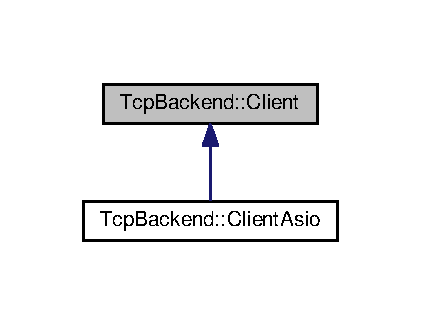
\includegraphics[width=202pt]{classTcpBackend_1_1Client__inherit__graph}
\end{center}
\end{figure}
\subsection*{Public Member Functions}
\begin{DoxyCompactItemize}
\item 
virtual \hyperlink{classTcpBackend_1_1Client_a0556d5f3d8a2894860d9073409f9eae0}{$\sim$\+Client} ()=default
\end{DoxyCompactItemize}


\subsection{Detailed Description}
Used to start a connection. 

See  

\subsection{Constructor \& Destructor Documentation}
\mbox{\Hypertarget{classTcpBackend_1_1Client_a0556d5f3d8a2894860d9073409f9eae0}\label{classTcpBackend_1_1Client_a0556d5f3d8a2894860d9073409f9eae0}} 
\index{Tcp\+Backend\+::\+Client@{Tcp\+Backend\+::\+Client}!````~Client@{$\sim$\+Client}}
\index{````~Client@{$\sim$\+Client}!Tcp\+Backend\+::\+Client@{Tcp\+Backend\+::\+Client}}
\subsubsection{\texorpdfstring{$\sim$\+Client()}{~Client()}}
{\footnotesize\ttfamily virtual Tcp\+Backend\+::\+Client\+::$\sim$\+Client (\begin{DoxyParamCaption}{ }\end{DoxyParamCaption})\hspace{0.3cm}{\ttfamily [virtual]}, {\ttfamily [default]}}



The documentation for this class was generated from the following file\+:\begin{DoxyCompactItemize}
\item 
src/\hyperlink{tcp__backend_8h}{tcp\+\_\+backend.\+h}\end{DoxyCompactItemize}

\hypertarget{classTcpBackend_1_1ClientAsio}{}\section{Tcp\+Backend\+:\+:Client\+Asio Class Reference}
\label{classTcpBackend_1_1ClientAsio}\index{Tcp\+Backend\+::\+Client\+Asio@{Tcp\+Backend\+::\+Client\+Asio}}


{\ttfamily \#include $<$tcp\+\_\+client\+\_\+asio.\+h$>$}



Inheritance diagram for Tcp\+Backend\+:\+:Client\+Asio\+:
\nopagebreak
\begin{figure}[H]
\begin{center}
\leavevmode
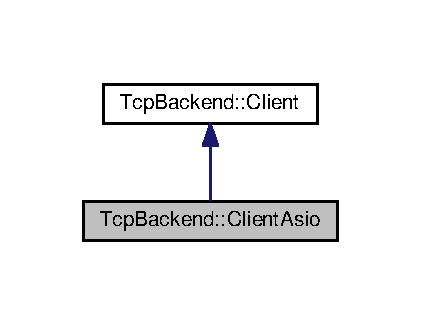
\includegraphics[width=202pt]{classTcpBackend_1_1ClientAsio__inherit__graph}
\end{center}
\end{figure}


Collaboration diagram for Tcp\+Backend\+:\+:Client\+Asio\+:
\nopagebreak
\begin{figure}[H]
\begin{center}
\leavevmode
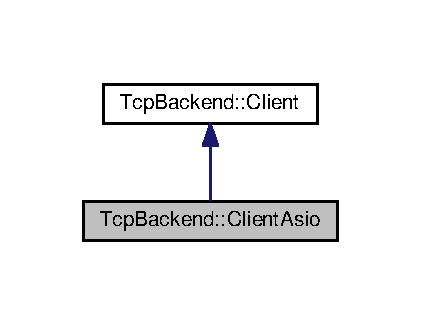
\includegraphics[width=202pt]{classTcpBackend_1_1ClientAsio__coll__graph}
\end{center}
\end{figure}
\subsection*{Public Member Functions}
\begin{DoxyCompactItemize}
\item 
\hyperlink{classTcpBackend_1_1ClientAsio_ac745c20f4213037c842d2d7c89397e84}{Client\+Asio} (asio\+::io\+\_\+service $\ast$io\+\_\+service, const std\+::string \&address, const std\+::string \&port, const \hyperlink{namespaceTcpBackend_afa30fa9a706436148fb2857a2174e625}{On\+Connected} \&on\+\_\+connected, const \hyperlink{namespaceTcpBackend_a17e8f044749312a6692cd0135565cbc4}{On\+Error} \&on\+\_\+error)
\end{DoxyCompactItemize}


\subsection{Constructor \& Destructor Documentation}
\mbox{\Hypertarget{classTcpBackend_1_1ClientAsio_ac745c20f4213037c842d2d7c89397e84}\label{classTcpBackend_1_1ClientAsio_ac745c20f4213037c842d2d7c89397e84}} 
\index{Tcp\+Backend\+::\+Client\+Asio@{Tcp\+Backend\+::\+Client\+Asio}!Client\+Asio@{Client\+Asio}}
\index{Client\+Asio@{Client\+Asio}!Tcp\+Backend\+::\+Client\+Asio@{Tcp\+Backend\+::\+Client\+Asio}}
\subsubsection{\texorpdfstring{Client\+Asio()}{ClientAsio()}}
{\footnotesize\ttfamily Tcp\+Backend\+::\+Client\+Asio\+::\+Client\+Asio (\begin{DoxyParamCaption}\item[{asio\+::io\+\_\+service $\ast$}]{io\+\_\+service,  }\item[{const std\+::string \&}]{address,  }\item[{const std\+::string \&}]{port,  }\item[{const \hyperlink{namespaceTcpBackend_afa30fa9a706436148fb2857a2174e625}{On\+Connected} \&}]{on\+\_\+connected,  }\item[{const \hyperlink{namespaceTcpBackend_a17e8f044749312a6692cd0135565cbc4}{On\+Error} \&}]{on\+\_\+error }\end{DoxyParamCaption})}



The documentation for this class was generated from the following files\+:\begin{DoxyCompactItemize}
\item 
src/backend\+\_\+asio/\hyperlink{tcp__client__asio_8h}{tcp\+\_\+client\+\_\+asio.\+h}\item 
src/backend\+\_\+asio/\hyperlink{tcp__client__asio_8cc}{tcp\+\_\+client\+\_\+asio.\+cc}\end{DoxyCompactItemize}

\hypertarget{classTcpBackend_1_1Connection}{}\section{Tcp\+Backend\+:\+:Connection Class Reference}
\label{classTcpBackend_1_1Connection}\index{Tcp\+Backend\+::\+Connection@{Tcp\+Backend\+::\+Connection}}


Represents a connection.  




{\ttfamily \#include $<$tcp\+\_\+backend.\+h$>$}



Inheritance diagram for Tcp\+Backend\+:\+:Connection\+:
\nopagebreak
\begin{figure}[H]
\begin{center}
\leavevmode
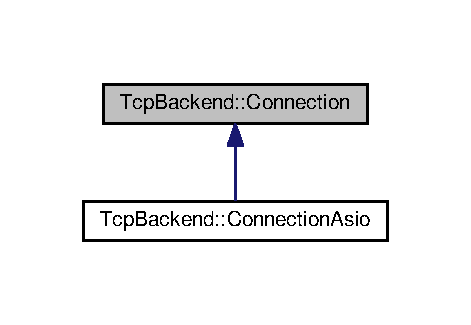
\includegraphics[width=226pt]{classTcpBackend_1_1Connection__inherit__graph}
\end{center}
\end{figure}
\subsection*{Public Member Functions}
\begin{DoxyCompactItemize}
\item 
virtual \hyperlink{classTcpBackend_1_1Connection_af9b388c0d9a4af734257da80bde24e30}{$\sim$\+Connection} ()=default
\item 
virtual void \hyperlink{classTcpBackend_1_1Connection_a653318aa6306df78e53af47ae9d05e04}{set\+\_\+callbacks} (const \hyperlink{namespaceTcpBackend_a2ce9b1a1f46bfa6c4b1ad38c8aa262a6}{On\+Disconnected} \&on\+\_\+disconnected, const \hyperlink{namespaceTcpBackend_a7d2c9f63e8017af705255d4ed08264a7}{On\+Read} \&on\+\_\+read, const \hyperlink{namespaceTcpBackend_a670c71abc926680e1ea574a5f3a99135}{On\+Write} \&on\+\_\+write, const \hyperlink{namespaceTcpBackend_a17e8f044749312a6692cd0135565cbc4}{On\+Error} \&on\+\_\+error)=0
\begin{DoxyCompactList}\small\item\em Set callbacks. \end{DoxyCompactList}\item 
virtual void \hyperlink{classTcpBackend_1_1Connection_a53c7544a1dc738fbf69d8081742f319c}{read} ()=0
\begin{DoxyCompactList}\small\item\em Starts read procedure (async) \end{DoxyCompactList}\item 
virtual void \hyperlink{classTcpBackend_1_1Connection_ab63e884129259b72a1d4614237048c46}{write} (const std\+::uint8\+\_\+t $\ast$buffer, int len)=0
\begin{DoxyCompactList}\small\item\em Starts write procedure (async) \end{DoxyCompactList}\item 
virtual void \hyperlink{classTcpBackend_1_1Connection_aa3cbc715deb54c286149457c7819f514}{close} ()=0
\begin{DoxyCompactList}\small\item\em Closes the connection. \end{DoxyCompactList}\end{DoxyCompactItemize}


\subsection{Detailed Description}
Represents a connection. 

Created by \hyperlink{classTcpBackend_1_1Client}{Client} or \hyperlink{classTcpBackend_1_1Server}{Server} when a connection has been established 

\subsection{Constructor \& Destructor Documentation}
\mbox{\Hypertarget{classTcpBackend_1_1Connection_af9b388c0d9a4af734257da80bde24e30}\label{classTcpBackend_1_1Connection_af9b388c0d9a4af734257da80bde24e30}} 
\index{Tcp\+Backend\+::\+Connection@{Tcp\+Backend\+::\+Connection}!````~Connection@{$\sim$\+Connection}}
\index{````~Connection@{$\sim$\+Connection}!Tcp\+Backend\+::\+Connection@{Tcp\+Backend\+::\+Connection}}
\subsubsection{\texorpdfstring{$\sim$\+Connection()}{~Connection()}}
{\footnotesize\ttfamily virtual Tcp\+Backend\+::\+Connection\+::$\sim$\+Connection (\begin{DoxyParamCaption}{ }\end{DoxyParamCaption})\hspace{0.3cm}{\ttfamily [virtual]}, {\ttfamily [default]}}



\subsection{Member Function Documentation}
\mbox{\Hypertarget{classTcpBackend_1_1Connection_aa3cbc715deb54c286149457c7819f514}\label{classTcpBackend_1_1Connection_aa3cbc715deb54c286149457c7819f514}} 
\index{Tcp\+Backend\+::\+Connection@{Tcp\+Backend\+::\+Connection}!close@{close}}
\index{close@{close}!Tcp\+Backend\+::\+Connection@{Tcp\+Backend\+::\+Connection}}
\subsubsection{\texorpdfstring{close()}{close()}}
{\footnotesize\ttfamily virtual void Tcp\+Backend\+::\+Connection\+::close (\begin{DoxyParamCaption}{ }\end{DoxyParamCaption})\hspace{0.3cm}{\ttfamily [pure virtual]}}



Closes the connection. 

Any ongoing async tasks will be aborted and the On\+Disconnected callback will be called either in this context or in a later context.

The \hyperlink{classTcpBackend_1_1Connection}{Connection} instance may only be deleted when the On\+Disconnected callback has been called. 

Implemented in \hyperlink{classTcpBackend_1_1ConnectionAsio_a4601c22735a27b1a835bfa73d9842848}{Tcp\+Backend\+::\+Connection\+Asio}.

\mbox{\Hypertarget{classTcpBackend_1_1Connection_a53c7544a1dc738fbf69d8081742f319c}\label{classTcpBackend_1_1Connection_a53c7544a1dc738fbf69d8081742f319c}} 
\index{Tcp\+Backend\+::\+Connection@{Tcp\+Backend\+::\+Connection}!read@{read}}
\index{read@{read}!Tcp\+Backend\+::\+Connection@{Tcp\+Backend\+::\+Connection}}
\subsubsection{\texorpdfstring{read()}{read()}}
{\footnotesize\ttfamily virtual void Tcp\+Backend\+::\+Connection\+::read (\begin{DoxyParamCaption}{ }\end{DoxyParamCaption})\hspace{0.3cm}{\ttfamily [pure virtual]}}



Starts read procedure (async) 

The On\+Read callback will be called when data has been read. 

Implemented in \hyperlink{classTcpBackend_1_1ConnectionAsio_a97faa75722fa9034ba03cf32512a6f22}{Tcp\+Backend\+::\+Connection\+Asio}.

\mbox{\Hypertarget{classTcpBackend_1_1Connection_a653318aa6306df78e53af47ae9d05e04}\label{classTcpBackend_1_1Connection_a653318aa6306df78e53af47ae9d05e04}} 
\index{Tcp\+Backend\+::\+Connection@{Tcp\+Backend\+::\+Connection}!set\+\_\+callbacks@{set\+\_\+callbacks}}
\index{set\+\_\+callbacks@{set\+\_\+callbacks}!Tcp\+Backend\+::\+Connection@{Tcp\+Backend\+::\+Connection}}
\subsubsection{\texorpdfstring{set\+\_\+callbacks()}{set\_callbacks()}}
{\footnotesize\ttfamily virtual void Tcp\+Backend\+::\+Connection\+::set\+\_\+callbacks (\begin{DoxyParamCaption}\item[{const \hyperlink{namespaceTcpBackend_a2ce9b1a1f46bfa6c4b1ad38c8aa262a6}{On\+Disconnected} \&}]{on\+\_\+disconnected,  }\item[{const \hyperlink{namespaceTcpBackend_a7d2c9f63e8017af705255d4ed08264a7}{On\+Read} \&}]{on\+\_\+read,  }\item[{const \hyperlink{namespaceTcpBackend_a670c71abc926680e1ea574a5f3a99135}{On\+Write} \&}]{on\+\_\+write,  }\item[{const \hyperlink{namespaceTcpBackend_a17e8f044749312a6692cd0135565cbc4}{On\+Error} \&}]{on\+\_\+error }\end{DoxyParamCaption})\hspace{0.3cm}{\ttfamily [pure virtual]}}



Set callbacks. 

These callbacks must be set before any read or write procedures are started.


\begin{DoxyParams}[1]{Parameters}
\mbox{\tt in}  & {\em on\+\_\+disconnected} & On\+Disconnected callback, see  \\
\hline
\mbox{\tt in}  & {\em on\+\_\+read} & On\+Read callback, see  \\
\hline
\mbox{\tt in}  & {\em on\+\_\+write} & On\+Write callback, see  \\
\hline
\mbox{\tt in}  & {\em on\+\_\+error} & On\+Error callback, see  \\
\hline
\end{DoxyParams}


Implemented in \hyperlink{classTcpBackend_1_1ConnectionAsio_aee6f9ded99c8382d3daaf2aa3d8890ee}{Tcp\+Backend\+::\+Connection\+Asio}.

\mbox{\Hypertarget{classTcpBackend_1_1Connection_ab63e884129259b72a1d4614237048c46}\label{classTcpBackend_1_1Connection_ab63e884129259b72a1d4614237048c46}} 
\index{Tcp\+Backend\+::\+Connection@{Tcp\+Backend\+::\+Connection}!write@{write}}
\index{write@{write}!Tcp\+Backend\+::\+Connection@{Tcp\+Backend\+::\+Connection}}
\subsubsection{\texorpdfstring{write()}{write()}}
{\footnotesize\ttfamily virtual void Tcp\+Backend\+::\+Connection\+::write (\begin{DoxyParamCaption}\item[{const std\+::uint8\+\_\+t $\ast$}]{buffer,  }\item[{int}]{len }\end{DoxyParamCaption})\hspace{0.3cm}{\ttfamily [pure virtual]}}



Starts write procedure (async) 


\begin{DoxyParams}[1]{Parameters}
\mbox{\tt in}  & {\em buffer} & The data to send \\
\hline
\mbox{\tt in}  & {\em len} & Length of data \\
\hline
\end{DoxyParams}


Implemented in \hyperlink{classTcpBackend_1_1ConnectionAsio_acca26b2c5f640224e1642e808138a580}{Tcp\+Backend\+::\+Connection\+Asio}.



The documentation for this class was generated from the following file\+:\begin{DoxyCompactItemize}
\item 
src/\hyperlink{tcp__backend_8h}{tcp\+\_\+backend.\+h}\end{DoxyCompactItemize}

\hypertarget{classTcpBackend_1_1ConnectionAsio}{}\section{Tcp\+Backend\+:\+:Connection\+Asio Class Reference}
\label{classTcpBackend_1_1ConnectionAsio}\index{Tcp\+Backend\+::\+Connection\+Asio@{Tcp\+Backend\+::\+Connection\+Asio}}


{\ttfamily \#include $<$tcp\+\_\+connection\+\_\+asio.\+h$>$}



Inheritance diagram for Tcp\+Backend\+:\+:Connection\+Asio\+:
\nopagebreak
\begin{figure}[H]
\begin{center}
\leavevmode
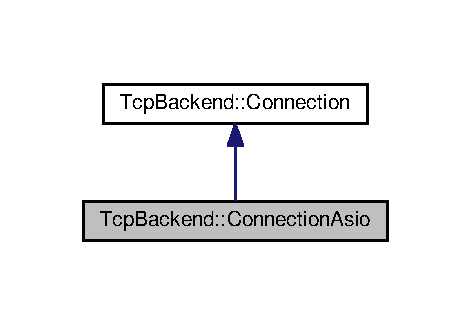
\includegraphics[width=226pt]{classTcpBackend_1_1ConnectionAsio__inherit__graph}
\end{center}
\end{figure}


Collaboration diagram for Tcp\+Backend\+:\+:Connection\+Asio\+:
\nopagebreak
\begin{figure}[H]
\begin{center}
\leavevmode
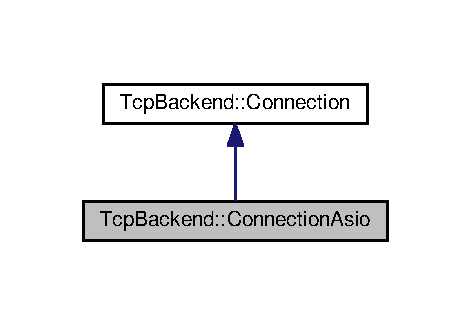
\includegraphics[width=226pt]{classTcpBackend_1_1ConnectionAsio__coll__graph}
\end{center}
\end{figure}
\subsection*{Public Member Functions}
\begin{DoxyCompactItemize}
\item 
\hyperlink{classTcpBackend_1_1ConnectionAsio_a736274fefc6ca4d83e03085fe2acbb7f}{Connection\+Asio} (asio\+::ip\+::tcp\+::socket socket)
\item 
void \hyperlink{classTcpBackend_1_1ConnectionAsio_aee6f9ded99c8382d3daaf2aa3d8890ee}{set\+\_\+callbacks} (const \hyperlink{namespaceTcpBackend_a2ce9b1a1f46bfa6c4b1ad38c8aa262a6}{On\+Disconnected} \&on\+\_\+disconnected, const \hyperlink{namespaceTcpBackend_a7d2c9f63e8017af705255d4ed08264a7}{On\+Read} \&on\+\_\+read, const \hyperlink{namespaceTcpBackend_a670c71abc926680e1ea574a5f3a99135}{On\+Write} \&on\+\_\+write, const \hyperlink{namespaceTcpBackend_a17e8f044749312a6692cd0135565cbc4}{On\+Error} \&on\+\_\+error) override
\begin{DoxyCompactList}\small\item\em Set callbacks. \end{DoxyCompactList}\item 
void \hyperlink{classTcpBackend_1_1ConnectionAsio_a97faa75722fa9034ba03cf32512a6f22}{read} () override
\begin{DoxyCompactList}\small\item\em Starts read procedure (async) \end{DoxyCompactList}\item 
void \hyperlink{classTcpBackend_1_1ConnectionAsio_acca26b2c5f640224e1642e808138a580}{write} (const std\+::uint8\+\_\+t $\ast$buffer, int len) override
\begin{DoxyCompactList}\small\item\em Starts write procedure (async) \end{DoxyCompactList}\item 
void \hyperlink{classTcpBackend_1_1ConnectionAsio_a4601c22735a27b1a835bfa73d9842848}{close} () override
\begin{DoxyCompactList}\small\item\em Closes the connection. \end{DoxyCompactList}\end{DoxyCompactItemize}


\subsection{Constructor \& Destructor Documentation}
\mbox{\Hypertarget{classTcpBackend_1_1ConnectionAsio_a736274fefc6ca4d83e03085fe2acbb7f}\label{classTcpBackend_1_1ConnectionAsio_a736274fefc6ca4d83e03085fe2acbb7f}} 
\index{Tcp\+Backend\+::\+Connection\+Asio@{Tcp\+Backend\+::\+Connection\+Asio}!Connection\+Asio@{Connection\+Asio}}
\index{Connection\+Asio@{Connection\+Asio}!Tcp\+Backend\+::\+Connection\+Asio@{Tcp\+Backend\+::\+Connection\+Asio}}
\subsubsection{\texorpdfstring{Connection\+Asio()}{ConnectionAsio()}}
{\footnotesize\ttfamily Tcp\+Backend\+::\+Connection\+Asio\+::\+Connection\+Asio (\begin{DoxyParamCaption}\item[{asio\+::ip\+::tcp\+::socket}]{socket }\end{DoxyParamCaption})}



\subsection{Member Function Documentation}
\mbox{\Hypertarget{classTcpBackend_1_1ConnectionAsio_a4601c22735a27b1a835bfa73d9842848}\label{classTcpBackend_1_1ConnectionAsio_a4601c22735a27b1a835bfa73d9842848}} 
\index{Tcp\+Backend\+::\+Connection\+Asio@{Tcp\+Backend\+::\+Connection\+Asio}!close@{close}}
\index{close@{close}!Tcp\+Backend\+::\+Connection\+Asio@{Tcp\+Backend\+::\+Connection\+Asio}}
\subsubsection{\texorpdfstring{close()}{close()}}
{\footnotesize\ttfamily void Tcp\+Backend\+::\+Connection\+Asio\+::close (\begin{DoxyParamCaption}{ }\end{DoxyParamCaption})\hspace{0.3cm}{\ttfamily [override]}, {\ttfamily [virtual]}}



Closes the connection. 

Any ongoing async tasks will be aborted and the On\+Disconnected callback will be called either in this context or in a later context.

The \hyperlink{classTcpBackend_1_1Connection}{Connection} instance may only be deleted when the On\+Disconnected callback has been called. 

Implements \hyperlink{classTcpBackend_1_1Connection_aa3cbc715deb54c286149457c7819f514}{Tcp\+Backend\+::\+Connection}.

\mbox{\Hypertarget{classTcpBackend_1_1ConnectionAsio_a97faa75722fa9034ba03cf32512a6f22}\label{classTcpBackend_1_1ConnectionAsio_a97faa75722fa9034ba03cf32512a6f22}} 
\index{Tcp\+Backend\+::\+Connection\+Asio@{Tcp\+Backend\+::\+Connection\+Asio}!read@{read}}
\index{read@{read}!Tcp\+Backend\+::\+Connection\+Asio@{Tcp\+Backend\+::\+Connection\+Asio}}
\subsubsection{\texorpdfstring{read()}{read()}}
{\footnotesize\ttfamily void Tcp\+Backend\+::\+Connection\+Asio\+::read (\begin{DoxyParamCaption}{ }\end{DoxyParamCaption})\hspace{0.3cm}{\ttfamily [override]}, {\ttfamily [virtual]}}



Starts read procedure (async) 

The On\+Read callback will be called when data has been read. 

Implements \hyperlink{classTcpBackend_1_1Connection_a53c7544a1dc738fbf69d8081742f319c}{Tcp\+Backend\+::\+Connection}.

\mbox{\Hypertarget{classTcpBackend_1_1ConnectionAsio_aee6f9ded99c8382d3daaf2aa3d8890ee}\label{classTcpBackend_1_1ConnectionAsio_aee6f9ded99c8382d3daaf2aa3d8890ee}} 
\index{Tcp\+Backend\+::\+Connection\+Asio@{Tcp\+Backend\+::\+Connection\+Asio}!set\+\_\+callbacks@{set\+\_\+callbacks}}
\index{set\+\_\+callbacks@{set\+\_\+callbacks}!Tcp\+Backend\+::\+Connection\+Asio@{Tcp\+Backend\+::\+Connection\+Asio}}
\subsubsection{\texorpdfstring{set\+\_\+callbacks()}{set\_callbacks()}}
{\footnotesize\ttfamily void Tcp\+Backend\+::\+Connection\+Asio\+::set\+\_\+callbacks (\begin{DoxyParamCaption}\item[{const \hyperlink{namespaceTcpBackend_a2ce9b1a1f46bfa6c4b1ad38c8aa262a6}{On\+Disconnected} \&}]{on\+\_\+disconnected,  }\item[{const \hyperlink{namespaceTcpBackend_a7d2c9f63e8017af705255d4ed08264a7}{On\+Read} \&}]{on\+\_\+read,  }\item[{const \hyperlink{namespaceTcpBackend_a670c71abc926680e1ea574a5f3a99135}{On\+Write} \&}]{on\+\_\+write,  }\item[{const \hyperlink{namespaceTcpBackend_a17e8f044749312a6692cd0135565cbc4}{On\+Error} \&}]{on\+\_\+error }\end{DoxyParamCaption})\hspace{0.3cm}{\ttfamily [override]}, {\ttfamily [virtual]}}



Set callbacks. 

These callbacks must be set before any read or write procedures are started.


\begin{DoxyParams}[1]{Parameters}
\mbox{\tt in}  & {\em on\+\_\+disconnected} & On\+Disconnected callback, see  \\
\hline
\mbox{\tt in}  & {\em on\+\_\+read} & On\+Read callback, see  \\
\hline
\mbox{\tt in}  & {\em on\+\_\+write} & On\+Write callback, see  \\
\hline
\mbox{\tt in}  & {\em on\+\_\+error} & On\+Error callback, see  \\
\hline
\end{DoxyParams}


Implements \hyperlink{classTcpBackend_1_1Connection_a653318aa6306df78e53af47ae9d05e04}{Tcp\+Backend\+::\+Connection}.

\mbox{\Hypertarget{classTcpBackend_1_1ConnectionAsio_acca26b2c5f640224e1642e808138a580}\label{classTcpBackend_1_1ConnectionAsio_acca26b2c5f640224e1642e808138a580}} 
\index{Tcp\+Backend\+::\+Connection\+Asio@{Tcp\+Backend\+::\+Connection\+Asio}!write@{write}}
\index{write@{write}!Tcp\+Backend\+::\+Connection\+Asio@{Tcp\+Backend\+::\+Connection\+Asio}}
\subsubsection{\texorpdfstring{write()}{write()}}
{\footnotesize\ttfamily void Tcp\+Backend\+::\+Connection\+Asio\+::write (\begin{DoxyParamCaption}\item[{const std\+::uint8\+\_\+t $\ast$}]{buffer,  }\item[{int}]{len }\end{DoxyParamCaption})\hspace{0.3cm}{\ttfamily [override]}, {\ttfamily [virtual]}}



Starts write procedure (async) 


\begin{DoxyParams}[1]{Parameters}
\mbox{\tt in}  & {\em buffer} & The data to send \\
\hline
\mbox{\tt in}  & {\em len} & Length of data \\
\hline
\end{DoxyParams}


Implements \hyperlink{classTcpBackend_1_1Connection_ab63e884129259b72a1d4614237048c46}{Tcp\+Backend\+::\+Connection}.



The documentation for this class was generated from the following files\+:\begin{DoxyCompactItemize}
\item 
src/backend\+\_\+asio/\hyperlink{tcp__connection__asio_8h}{tcp\+\_\+connection\+\_\+asio.\+h}\item 
src/backend\+\_\+asio/\hyperlink{tcp__connection__asio_8cc}{tcp\+\_\+connection\+\_\+asio.\+cc}\end{DoxyCompactItemize}

\hypertarget{structProtocol_1_1Request}{}\section{Protocol\+:\+:Request Struct Reference}
\label{structProtocol_1_1Request}\index{Protocol\+::\+Request@{Protocol\+::\+Request}}


{\ttfamily \#include $<$protocol.\+h$>$}

\subsection*{Data Fields}
\begin{DoxyCompactItemize}
\item 
std\+::complex$<$ double $>$ \hyperlink{structProtocol_1_1Request_a4a4739df28bbb9a1252dedeb5f918db8}{min\+\_\+c}
\item 
std\+::complex$<$ double $>$ \hyperlink{structProtocol_1_1Request_a65b9e26893f8ab218ded9bf88f7b7003}{max\+\_\+c}
\item 
std\+::uint32\+\_\+t \hyperlink{structProtocol_1_1Request_a44b8822481390a24fb2dc4b3dbb50873}{image\+\_\+width}
\item 
std\+::uint32\+\_\+t \hyperlink{structProtocol_1_1Request_adced81ab70e49c64830fe4ac4fc2c3c5}{image\+\_\+height}
\item 
std\+::uint32\+\_\+t \hyperlink{structProtocol_1_1Request_a1ab4bee193a4599f5db9281fa41f31e2}{max\+\_\+iter}
\end{DoxyCompactItemize}


\subsection{Field Documentation}
\mbox{\Hypertarget{structProtocol_1_1Request_adced81ab70e49c64830fe4ac4fc2c3c5}\label{structProtocol_1_1Request_adced81ab70e49c64830fe4ac4fc2c3c5}} 
\index{Protocol\+::\+Request@{Protocol\+::\+Request}!image\+\_\+height@{image\+\_\+height}}
\index{image\+\_\+height@{image\+\_\+height}!Protocol\+::\+Request@{Protocol\+::\+Request}}
\subsubsection{\texorpdfstring{image\+\_\+height}{image\_height}}
{\footnotesize\ttfamily std\+::uint32\+\_\+t Protocol\+::\+Request\+::image\+\_\+height}

\mbox{\Hypertarget{structProtocol_1_1Request_a44b8822481390a24fb2dc4b3dbb50873}\label{structProtocol_1_1Request_a44b8822481390a24fb2dc4b3dbb50873}} 
\index{Protocol\+::\+Request@{Protocol\+::\+Request}!image\+\_\+width@{image\+\_\+width}}
\index{image\+\_\+width@{image\+\_\+width}!Protocol\+::\+Request@{Protocol\+::\+Request}}
\subsubsection{\texorpdfstring{image\+\_\+width}{image\_width}}
{\footnotesize\ttfamily std\+::uint32\+\_\+t Protocol\+::\+Request\+::image\+\_\+width}

\mbox{\Hypertarget{structProtocol_1_1Request_a65b9e26893f8ab218ded9bf88f7b7003}\label{structProtocol_1_1Request_a65b9e26893f8ab218ded9bf88f7b7003}} 
\index{Protocol\+::\+Request@{Protocol\+::\+Request}!max\+\_\+c@{max\+\_\+c}}
\index{max\+\_\+c@{max\+\_\+c}!Protocol\+::\+Request@{Protocol\+::\+Request}}
\subsubsection{\texorpdfstring{max\+\_\+c}{max\_c}}
{\footnotesize\ttfamily std\+::complex$<$double$>$ Protocol\+::\+Request\+::max\+\_\+c}

\mbox{\Hypertarget{structProtocol_1_1Request_a1ab4bee193a4599f5db9281fa41f31e2}\label{structProtocol_1_1Request_a1ab4bee193a4599f5db9281fa41f31e2}} 
\index{Protocol\+::\+Request@{Protocol\+::\+Request}!max\+\_\+iter@{max\+\_\+iter}}
\index{max\+\_\+iter@{max\+\_\+iter}!Protocol\+::\+Request@{Protocol\+::\+Request}}
\subsubsection{\texorpdfstring{max\+\_\+iter}{max\_iter}}
{\footnotesize\ttfamily std\+::uint32\+\_\+t Protocol\+::\+Request\+::max\+\_\+iter}

\mbox{\Hypertarget{structProtocol_1_1Request_a4a4739df28bbb9a1252dedeb5f918db8}\label{structProtocol_1_1Request_a4a4739df28bbb9a1252dedeb5f918db8}} 
\index{Protocol\+::\+Request@{Protocol\+::\+Request}!min\+\_\+c@{min\+\_\+c}}
\index{min\+\_\+c@{min\+\_\+c}!Protocol\+::\+Request@{Protocol\+::\+Request}}
\subsubsection{\texorpdfstring{min\+\_\+c}{min\_c}}
{\footnotesize\ttfamily std\+::complex$<$double$>$ Protocol\+::\+Request\+::min\+\_\+c}



The documentation for this struct was generated from the following file\+:\begin{DoxyCompactItemize}
\item 
src/\hyperlink{protocol_8h}{protocol.\+h}\end{DoxyCompactItemize}

\hypertarget{structProtocol_1_1Response}{}\section{Protocol\+:\+:Response Struct Reference}
\label{structProtocol_1_1Response}\index{Protocol\+::\+Response@{Protocol\+::\+Response}}


{\ttfamily \#include $<$protocol.\+h$>$}

\subsection*{Data Fields}
\begin{DoxyCompactItemize}
\item 
std\+::vector$<$ std\+::uint8\+\_\+t $>$ \hyperlink{structProtocol_1_1Response_a5581498781fbccae5bb6082a37a23e6b}{pixels}
\item 
bool \hyperlink{structProtocol_1_1Response_a494170c5e2442a8d35e1227f40683ec1}{last\+\_\+message}
\end{DoxyCompactItemize}


\subsection{Field Documentation}
\mbox{\Hypertarget{structProtocol_1_1Response_a494170c5e2442a8d35e1227f40683ec1}\label{structProtocol_1_1Response_a494170c5e2442a8d35e1227f40683ec1}} 
\index{Protocol\+::\+Response@{Protocol\+::\+Response}!last\+\_\+message@{last\+\_\+message}}
\index{last\+\_\+message@{last\+\_\+message}!Protocol\+::\+Response@{Protocol\+::\+Response}}
\subsubsection{\texorpdfstring{last\+\_\+message}{last\_message}}
{\footnotesize\ttfamily bool Protocol\+::\+Response\+::last\+\_\+message}

\mbox{\Hypertarget{structProtocol_1_1Response_a5581498781fbccae5bb6082a37a23e6b}\label{structProtocol_1_1Response_a5581498781fbccae5bb6082a37a23e6b}} 
\index{Protocol\+::\+Response@{Protocol\+::\+Response}!pixels@{pixels}}
\index{pixels@{pixels}!Protocol\+::\+Response@{Protocol\+::\+Response}}
\subsubsection{\texorpdfstring{pixels}{pixels}}
{\footnotesize\ttfamily std\+::vector$<$std\+::uint8\+\_\+t$>$ Protocol\+::\+Response\+::pixels}



The documentation for this struct was generated from the following file\+:\begin{DoxyCompactItemize}
\item 
src/\hyperlink{protocol_8h}{protocol.\+h}\end{DoxyCompactItemize}

\hypertarget{classTcpBackend_1_1Server}{}\section{Tcp\+Backend\+:\+:Server Class Reference}
\label{classTcpBackend_1_1Server}\index{Tcp\+Backend\+::\+Server@{Tcp\+Backend\+::\+Server}}


Used to accept new connections.  




{\ttfamily \#include $<$tcp\+\_\+backend.\+h$>$}



Inheritance diagram for Tcp\+Backend\+:\+:Server\+:
\nopagebreak
\begin{figure}[H]
\begin{center}
\leavevmode
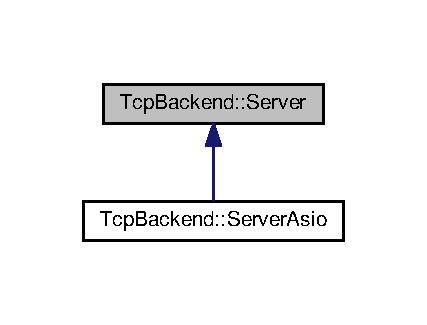
\includegraphics[width=205pt]{classTcpBackend_1_1Server__inherit__graph}
\end{center}
\end{figure}
\subsection*{Public Member Functions}
\begin{DoxyCompactItemize}
\item 
virtual \hyperlink{classTcpBackend_1_1Server_a567fe5cf7bc9ed07eec98bc21ba5b294}{$\sim$\+Server} ()=default
\item 
virtual void \hyperlink{classTcpBackend_1_1Server_aab685a052c45a25ecc9a30ec14bf91e9}{accept} ()=0
\begin{DoxyCompactList}\small\item\em Start accept procedure (async) \end{DoxyCompactList}\end{DoxyCompactItemize}


\subsection{Detailed Description}
Used to accept new connections. 

See  

\subsection{Constructor \& Destructor Documentation}
\mbox{\Hypertarget{classTcpBackend_1_1Server_a567fe5cf7bc9ed07eec98bc21ba5b294}\label{classTcpBackend_1_1Server_a567fe5cf7bc9ed07eec98bc21ba5b294}} 
\index{Tcp\+Backend\+::\+Server@{Tcp\+Backend\+::\+Server}!````~Server@{$\sim$\+Server}}
\index{````~Server@{$\sim$\+Server}!Tcp\+Backend\+::\+Server@{Tcp\+Backend\+::\+Server}}
\subsubsection{\texorpdfstring{$\sim$\+Server()}{~Server()}}
{\footnotesize\ttfamily virtual Tcp\+Backend\+::\+Server\+::$\sim$\+Server (\begin{DoxyParamCaption}{ }\end{DoxyParamCaption})\hspace{0.3cm}{\ttfamily [virtual]}, {\ttfamily [default]}}



\subsection{Member Function Documentation}
\mbox{\Hypertarget{classTcpBackend_1_1Server_aab685a052c45a25ecc9a30ec14bf91e9}\label{classTcpBackend_1_1Server_aab685a052c45a25ecc9a30ec14bf91e9}} 
\index{Tcp\+Backend\+::\+Server@{Tcp\+Backend\+::\+Server}!accept@{accept}}
\index{accept@{accept}!Tcp\+Backend\+::\+Server@{Tcp\+Backend\+::\+Server}}
\subsubsection{\texorpdfstring{accept()}{accept()}}
{\footnotesize\ttfamily virtual void Tcp\+Backend\+::\+Server\+::accept (\begin{DoxyParamCaption}{ }\end{DoxyParamCaption})\hspace{0.3cm}{\ttfamily [pure virtual]}}



Start accept procedure (async) 



Implemented in \hyperlink{classTcpBackend_1_1ServerAsio_adc51e0fe964cfaf725d4c1b999dd36c1}{Tcp\+Backend\+::\+Server\+Asio}.



The documentation for this class was generated from the following file\+:\begin{DoxyCompactItemize}
\item 
src/\hyperlink{tcp__backend_8h}{tcp\+\_\+backend.\+h}\end{DoxyCompactItemize}

\hypertarget{classTcpBackend_1_1ServerAsio}{}\section{Tcp\+Backend\+:\+:Server\+Asio Class Reference}
\label{classTcpBackend_1_1ServerAsio}\index{Tcp\+Backend\+::\+Server\+Asio@{Tcp\+Backend\+::\+Server\+Asio}}


{\ttfamily \#include $<$tcp\+\_\+server\+\_\+asio.\+h$>$}



Inheritance diagram for Tcp\+Backend\+:\+:Server\+Asio\+:
\nopagebreak
\begin{figure}[H]
\begin{center}
\leavevmode
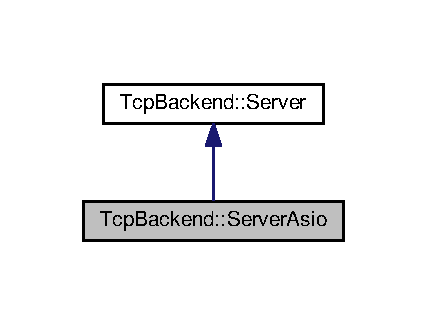
\includegraphics[width=205pt]{classTcpBackend_1_1ServerAsio__inherit__graph}
\end{center}
\end{figure}


Collaboration diagram for Tcp\+Backend\+:\+:Server\+Asio\+:
\nopagebreak
\begin{figure}[H]
\begin{center}
\leavevmode
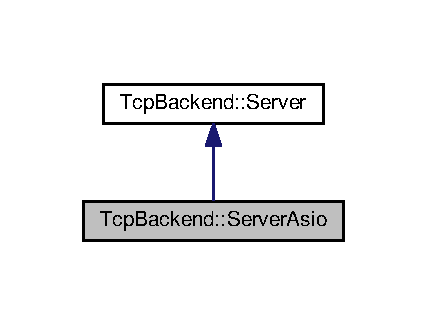
\includegraphics[width=205pt]{classTcpBackend_1_1ServerAsio__coll__graph}
\end{center}
\end{figure}
\subsection*{Public Member Functions}
\begin{DoxyCompactItemize}
\item 
\hyperlink{classTcpBackend_1_1ServerAsio_ade8fcf1b5853bcde95a7ddcf40f6de12}{Server\+Asio} (asio\+::io\+\_\+service $\ast$io\+\_\+service, std\+::uint16\+\_\+t port, const \hyperlink{namespaceTcpBackend_a8aed04c0b1d33eb06aec746da4452484}{On\+Accept} \&on\+\_\+accept)
\item 
void \hyperlink{classTcpBackend_1_1ServerAsio_adc51e0fe964cfaf725d4c1b999dd36c1}{accept} () override
\begin{DoxyCompactList}\small\item\em Start accept procedure (async) \end{DoxyCompactList}\end{DoxyCompactItemize}


\subsection{Constructor \& Destructor Documentation}
\mbox{\Hypertarget{classTcpBackend_1_1ServerAsio_ade8fcf1b5853bcde95a7ddcf40f6de12}\label{classTcpBackend_1_1ServerAsio_ade8fcf1b5853bcde95a7ddcf40f6de12}} 
\index{Tcp\+Backend\+::\+Server\+Asio@{Tcp\+Backend\+::\+Server\+Asio}!Server\+Asio@{Server\+Asio}}
\index{Server\+Asio@{Server\+Asio}!Tcp\+Backend\+::\+Server\+Asio@{Tcp\+Backend\+::\+Server\+Asio}}
\subsubsection{\texorpdfstring{Server\+Asio()}{ServerAsio()}}
{\footnotesize\ttfamily Tcp\+Backend\+::\+Server\+Asio\+::\+Server\+Asio (\begin{DoxyParamCaption}\item[{asio\+::io\+\_\+service $\ast$}]{io\+\_\+service,  }\item[{std\+::uint16\+\_\+t}]{port,  }\item[{const \hyperlink{namespaceTcpBackend_a8aed04c0b1d33eb06aec746da4452484}{On\+Accept} \&}]{on\+\_\+accept }\end{DoxyParamCaption})}



\subsection{Member Function Documentation}
\mbox{\Hypertarget{classTcpBackend_1_1ServerAsio_adc51e0fe964cfaf725d4c1b999dd36c1}\label{classTcpBackend_1_1ServerAsio_adc51e0fe964cfaf725d4c1b999dd36c1}} 
\index{Tcp\+Backend\+::\+Server\+Asio@{Tcp\+Backend\+::\+Server\+Asio}!accept@{accept}}
\index{accept@{accept}!Tcp\+Backend\+::\+Server\+Asio@{Tcp\+Backend\+::\+Server\+Asio}}
\subsubsection{\texorpdfstring{accept()}{accept()}}
{\footnotesize\ttfamily void Tcp\+Backend\+::\+Server\+Asio\+::accept (\begin{DoxyParamCaption}{ }\end{DoxyParamCaption})\hspace{0.3cm}{\ttfamily [override]}, {\ttfamily [virtual]}}



Start accept procedure (async) 



Implements \hyperlink{classTcpBackend_1_1Server_aab685a052c45a25ecc9a30ec14bf91e9}{Tcp\+Backend\+::\+Server}.



The documentation for this class was generated from the following files\+:\begin{DoxyCompactItemize}
\item 
src/backend\+\_\+asio/\hyperlink{tcp__server__asio_8h}{tcp\+\_\+server\+\_\+asio.\+h}\item 
src/backend\+\_\+asio/\hyperlink{tcp__server__asio_8cc}{tcp\+\_\+server\+\_\+asio.\+cc}\end{DoxyCompactItemize}

\hypertarget{structSession}{}\section{Session Struct Reference}
\label{structSession}\index{Session@{Session}}


Collaboration diagram for Session\+:
\nopagebreak
\begin{figure}[H]
\begin{center}
\leavevmode
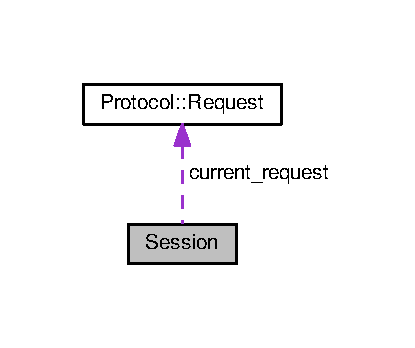
\includegraphics[width=199pt]{structSession__coll__graph}
\end{center}
\end{figure}
\subsection*{Data Fields}
\begin{DoxyCompactItemize}
\item 
std\+::unique\+\_\+ptr$<$ \hyperlink{classTcpBackend_1_1Connection}{Tcp\+Backend\+::\+Connection} $>$ \hyperlink{structSession_a55ef585b763a1a3e645b70826bbdb5ee}{connection}
\item 
bool \hyperlink{structSession_a7136254f114d887ab73172b395c040d5}{request\+\_\+ongoing}
\item 
\hyperlink{structProtocol_1_1Request}{Protocol\+::\+Request} \hyperlink{structSession_a1358d19f1cfc7e2ac6c2c6ad51ef2f42}{current\+\_\+request}
\item 
std\+::vector$<$ std\+::uint8\+\_\+t $>$ \hyperlink{structSession_a8000e4b6e8ab34810d9771a8d7bf59e6}{current\+\_\+pixels}
\end{DoxyCompactItemize}


\subsection{Field Documentation}
\mbox{\Hypertarget{structSession_a55ef585b763a1a3e645b70826bbdb5ee}\label{structSession_a55ef585b763a1a3e645b70826bbdb5ee}} 
\index{Session@{Session}!connection@{connection}}
\index{connection@{connection}!Session@{Session}}
\subsubsection{\texorpdfstring{connection}{connection}}
{\footnotesize\ttfamily std\+::unique\+\_\+ptr$<$\hyperlink{classTcpBackend_1_1Connection}{Tcp\+Backend\+::\+Connection}$>$ Session\+::connection}

\mbox{\Hypertarget{structSession_a8000e4b6e8ab34810d9771a8d7bf59e6}\label{structSession_a8000e4b6e8ab34810d9771a8d7bf59e6}} 
\index{Session@{Session}!current\+\_\+pixels@{current\+\_\+pixels}}
\index{current\+\_\+pixels@{current\+\_\+pixels}!Session@{Session}}
\subsubsection{\texorpdfstring{current\+\_\+pixels}{current\_pixels}}
{\footnotesize\ttfamily std\+::vector$<$std\+::uint8\+\_\+t$>$ Session\+::current\+\_\+pixels}

\mbox{\Hypertarget{structSession_a1358d19f1cfc7e2ac6c2c6ad51ef2f42}\label{structSession_a1358d19f1cfc7e2ac6c2c6ad51ef2f42}} 
\index{Session@{Session}!current\+\_\+request@{current\+\_\+request}}
\index{current\+\_\+request@{current\+\_\+request}!Session@{Session}}
\subsubsection{\texorpdfstring{current\+\_\+request}{current\_request}}
{\footnotesize\ttfamily \hyperlink{structProtocol_1_1Request}{Protocol\+::\+Request} Session\+::current\+\_\+request}

\mbox{\Hypertarget{structSession_a7136254f114d887ab73172b395c040d5}\label{structSession_a7136254f114d887ab73172b395c040d5}} 
\index{Session@{Session}!request\+\_\+ongoing@{request\+\_\+ongoing}}
\index{request\+\_\+ongoing@{request\+\_\+ongoing}!Session@{Session}}
\subsubsection{\texorpdfstring{request\+\_\+ongoing}{request\_ongoing}}
{\footnotesize\ttfamily bool Session\+::request\+\_\+ongoing}



The documentation for this struct was generated from the following file\+:\begin{DoxyCompactItemize}
\item 
src/\hyperlink{pmp__client_8cc}{pmp\+\_\+client.\+cc}\end{DoxyCompactItemize}

\hypertarget{classTcpConnectionEpoll}{}\section{Tcp\+Connection\+Epoll Class Reference}
\label{classTcpConnectionEpoll}\index{Tcp\+Connection\+Epoll@{Tcp\+Connection\+Epoll}}


{\ttfamily \#include $<$tcp\+\_\+connection\+\_\+epoll.\+h$>$}



Inheritance diagram for Tcp\+Connection\+Epoll\+:
\nopagebreak
\begin{figure}[H]
\begin{center}
\leavevmode
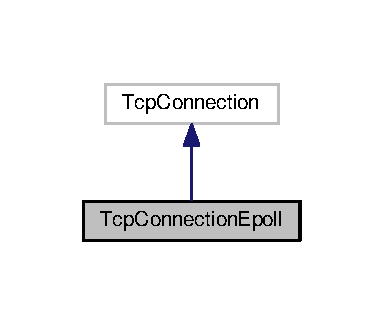
\includegraphics[width=184pt]{classTcpConnectionEpoll__inherit__graph}
\end{center}
\end{figure}


Collaboration diagram for Tcp\+Connection\+Epoll\+:
\nopagebreak
\begin{figure}[H]
\begin{center}
\leavevmode
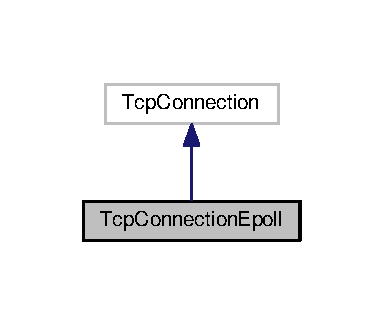
\includegraphics[width=184pt]{classTcpConnectionEpoll__coll__graph}
\end{center}
\end{figure}
\subsection*{Public Member Functions}
\begin{DoxyCompactItemize}
\item 
\hyperlink{classTcpConnectionEpoll_a8a0d4fe2dc75d4e6f29f0221aeb16516}{Tcp\+Connection\+Epoll} (int socket\+\_\+fd)
\item 
void \hyperlink{classTcpConnectionEpoll_a6109a1ddd496e5307888d2c70fffc2c6}{close} () override
\end{DoxyCompactItemize}


\subsection{Constructor \& Destructor Documentation}
\mbox{\Hypertarget{classTcpConnectionEpoll_a8a0d4fe2dc75d4e6f29f0221aeb16516}\label{classTcpConnectionEpoll_a8a0d4fe2dc75d4e6f29f0221aeb16516}} 
\index{Tcp\+Connection\+Epoll@{Tcp\+Connection\+Epoll}!Tcp\+Connection\+Epoll@{Tcp\+Connection\+Epoll}}
\index{Tcp\+Connection\+Epoll@{Tcp\+Connection\+Epoll}!Tcp\+Connection\+Epoll@{Tcp\+Connection\+Epoll}}
\subsubsection{\texorpdfstring{Tcp\+Connection\+Epoll()}{TcpConnectionEpoll()}}
{\footnotesize\ttfamily Tcp\+Connection\+Epoll\+::\+Tcp\+Connection\+Epoll (\begin{DoxyParamCaption}\item[{int}]{socket\+\_\+fd }\end{DoxyParamCaption})}



\subsection{Member Function Documentation}
\mbox{\Hypertarget{classTcpConnectionEpoll_a6109a1ddd496e5307888d2c70fffc2c6}\label{classTcpConnectionEpoll_a6109a1ddd496e5307888d2c70fffc2c6}} 
\index{Tcp\+Connection\+Epoll@{Tcp\+Connection\+Epoll}!close@{close}}
\index{close@{close}!Tcp\+Connection\+Epoll@{Tcp\+Connection\+Epoll}}
\subsubsection{\texorpdfstring{close()}{close()}}
{\footnotesize\ttfamily void Tcp\+Connection\+Epoll\+::close (\begin{DoxyParamCaption}{ }\end{DoxyParamCaption})\hspace{0.3cm}{\ttfamily [override]}}



The documentation for this class was generated from the following files\+:\begin{DoxyCompactItemize}
\item 
src/backend\+\_\+epoll/\hyperlink{tcp__connection__epoll_8h}{tcp\+\_\+connection\+\_\+epoll.\+h}\item 
src/backend\+\_\+epoll/\hyperlink{tcp__connection__epoll_8cc}{tcp\+\_\+connection\+\_\+epoll.\+cc}\end{DoxyCompactItemize}

\hypertarget{classTcpServerEpoll}{}\section{Tcp\+Server\+Epoll Class Reference}
\label{classTcpServerEpoll}\index{Tcp\+Server\+Epoll@{Tcp\+Server\+Epoll}}


{\ttfamily \#include $<$tcp\+\_\+server\+\_\+epoll.\+h$>$}



Inheritance diagram for Tcp\+Server\+Epoll\+:
\nopagebreak
\begin{figure}[H]
\begin{center}
\leavevmode
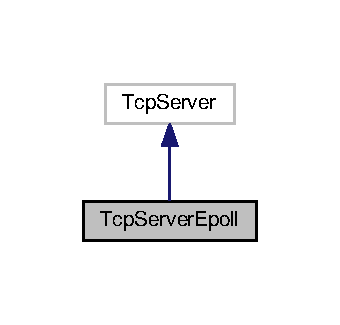
\includegraphics[width=163pt]{classTcpServerEpoll__inherit__graph}
\end{center}
\end{figure}


Collaboration diagram for Tcp\+Server\+Epoll\+:
\nopagebreak
\begin{figure}[H]
\begin{center}
\leavevmode
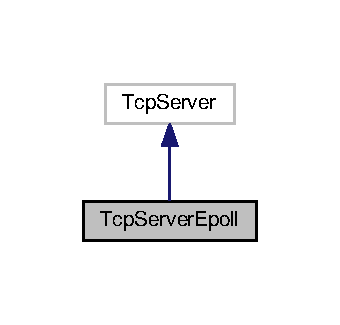
\includegraphics[width=163pt]{classTcpServerEpoll__coll__graph}
\end{center}
\end{figure}
\subsection*{Public Member Functions}
\begin{DoxyCompactItemize}
\item 
\hyperlink{classTcpServerEpoll_aaf7ecde753d57703ac9fbf21e489ea22}{Tcp\+Server\+Epoll} (int socket\+\_\+fd, const On\+Accept \&on\+\_\+accept)
\item 
void \hyperlink{classTcpServerEpoll_a03ad291fa33bf9749e9b940337c56064}{start} () override
\end{DoxyCompactItemize}


\subsection{Constructor \& Destructor Documentation}
\mbox{\Hypertarget{classTcpServerEpoll_aaf7ecde753d57703ac9fbf21e489ea22}\label{classTcpServerEpoll_aaf7ecde753d57703ac9fbf21e489ea22}} 
\index{Tcp\+Server\+Epoll@{Tcp\+Server\+Epoll}!Tcp\+Server\+Epoll@{Tcp\+Server\+Epoll}}
\index{Tcp\+Server\+Epoll@{Tcp\+Server\+Epoll}!Tcp\+Server\+Epoll@{Tcp\+Server\+Epoll}}
\subsubsection{\texorpdfstring{Tcp\+Server\+Epoll()}{TcpServerEpoll()}}
{\footnotesize\ttfamily Tcp\+Server\+Epoll\+::\+Tcp\+Server\+Epoll (\begin{DoxyParamCaption}\item[{int}]{socket\+\_\+fd,  }\item[{const On\+Accept \&}]{on\+\_\+accept }\end{DoxyParamCaption})}



\subsection{Member Function Documentation}
\mbox{\Hypertarget{classTcpServerEpoll_a03ad291fa33bf9749e9b940337c56064}\label{classTcpServerEpoll_a03ad291fa33bf9749e9b940337c56064}} 
\index{Tcp\+Server\+Epoll@{Tcp\+Server\+Epoll}!start@{start}}
\index{start@{start}!Tcp\+Server\+Epoll@{Tcp\+Server\+Epoll}}
\subsubsection{\texorpdfstring{start()}{start()}}
{\footnotesize\ttfamily void Tcp\+Server\+Epoll\+::start (\begin{DoxyParamCaption}{ }\end{DoxyParamCaption})\hspace{0.3cm}{\ttfamily [override]}}



The documentation for this class was generated from the following files\+:\begin{DoxyCompactItemize}
\item 
src/backend\+\_\+epoll/\hyperlink{tcp__server__epoll_8h}{tcp\+\_\+server\+\_\+epoll.\+h}\item 
src/backend\+\_\+epoll/\hyperlink{tcp__server__epoll_8cc}{tcp\+\_\+server\+\_\+epoll.\+cc}\end{DoxyCompactItemize}

\chapter{File Documentation}
\hypertarget{tcp__backend__asio_8cc}{}\section{src/backend\+\_\+asio/tcp\+\_\+backend\+\_\+asio.cc File Reference}
\label{tcp__backend__asio_8cc}\index{src/backend\+\_\+asio/tcp\+\_\+backend\+\_\+asio.\+cc@{src/backend\+\_\+asio/tcp\+\_\+backend\+\_\+asio.\+cc}}
{\ttfamily \#include \char`\"{}tcp\+\_\+backend.\+h\char`\"{}}\newline
{\ttfamily \#include $<$asio.\+hpp$>$}\newline
{\ttfamily \#include \char`\"{}tcp\+\_\+connection\+\_\+asio.\+h\char`\"{}}\newline
{\ttfamily \#include \char`\"{}tcp\+\_\+client\+\_\+asio.\+h\char`\"{}}\newline
{\ttfamily \#include \char`\"{}tcp\+\_\+server\+\_\+asio.\+h\char`\"{}}\newline
Include dependency graph for tcp\+\_\+backend\+\_\+asio.\+cc\+:
\nopagebreak
\begin{figure}[H]
\begin{center}
\leavevmode
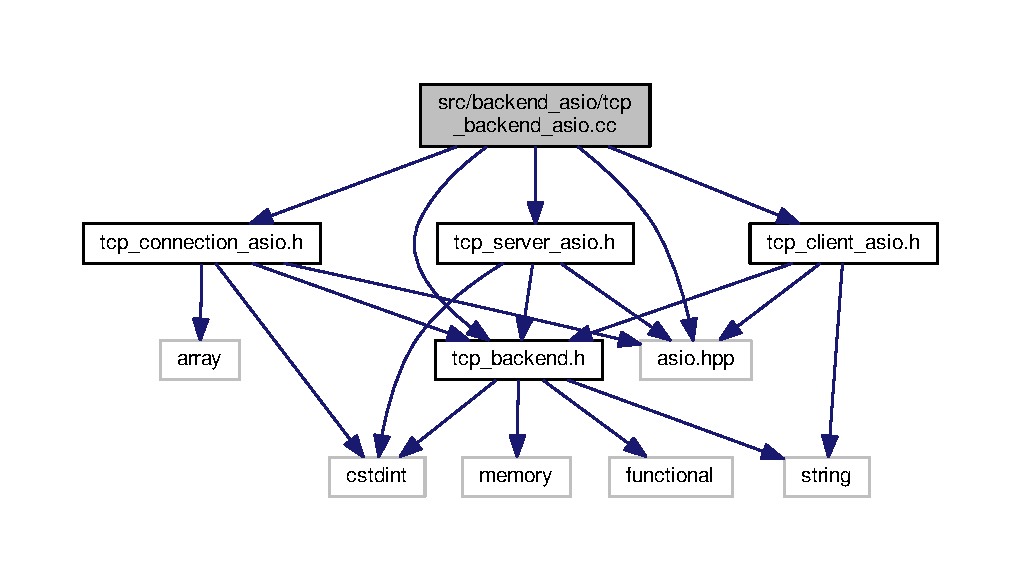
\includegraphics[width=350pt]{tcp__backend__asio_8cc__incl}
\end{center}
\end{figure}
\subsection*{Namespaces}
\begin{DoxyCompactItemize}
\item 
 \hyperlink{namespaceTcpBackend}{Tcp\+Backend}
\end{DoxyCompactItemize}
\subsection*{Functions}
\begin{DoxyCompactItemize}
\item 
std\+::unique\+\_\+ptr$<$ Client $>$ \hyperlink{namespaceTcpBackend_ac561d1ab714a1b76b3db75b205dd4f84}{Tcp\+Backend\+::create\+\_\+client} (const std\+::string \&address, const std\+::string \&port, const On\+Connected \&on\+\_\+connected, const On\+Error \&on\+\_\+error)
\begin{DoxyCompactList}\small\item\em Creates a T\+CP client. \end{DoxyCompactList}\item 
std\+::unique\+\_\+ptr$<$ Server $>$ \hyperlink{namespaceTcpBackend_ad25ce62084f2e8ec8e6bd07d7510b7f2}{Tcp\+Backend\+::create\+\_\+server} (std\+::uint16\+\_\+t port, const On\+Accept \&on\+\_\+accept)
\begin{DoxyCompactList}\small\item\em Creates a T\+CP server. \end{DoxyCompactList}\item 
void \hyperlink{namespaceTcpBackend_ad949ba412696b6c7484f981fcb36a705}{Tcp\+Backend\+::run} ()
\begin{DoxyCompactList}\small\item\em Run the T\+CP backend. \end{DoxyCompactList}\end{DoxyCompactItemize}

\hypertarget{tcp__client__asio_8cc}{}\section{src/backend\+\_\+asio/tcp\+\_\+client\+\_\+asio.cc File Reference}
\label{tcp__client__asio_8cc}\index{src/backend\+\_\+asio/tcp\+\_\+client\+\_\+asio.\+cc@{src/backend\+\_\+asio/tcp\+\_\+client\+\_\+asio.\+cc}}
{\ttfamily \#include \char`\"{}tcp\+\_\+client\+\_\+asio.\+h\char`\"{}}\newline
{\ttfamily \#include $<$memory$>$}\newline
{\ttfamily \#include \char`\"{}tcp\+\_\+connection\+\_\+asio.\+h\char`\"{}}\newline
Include dependency graph for tcp\+\_\+client\+\_\+asio.\+cc\+:
\nopagebreak
\begin{figure}[H]
\begin{center}
\leavevmode
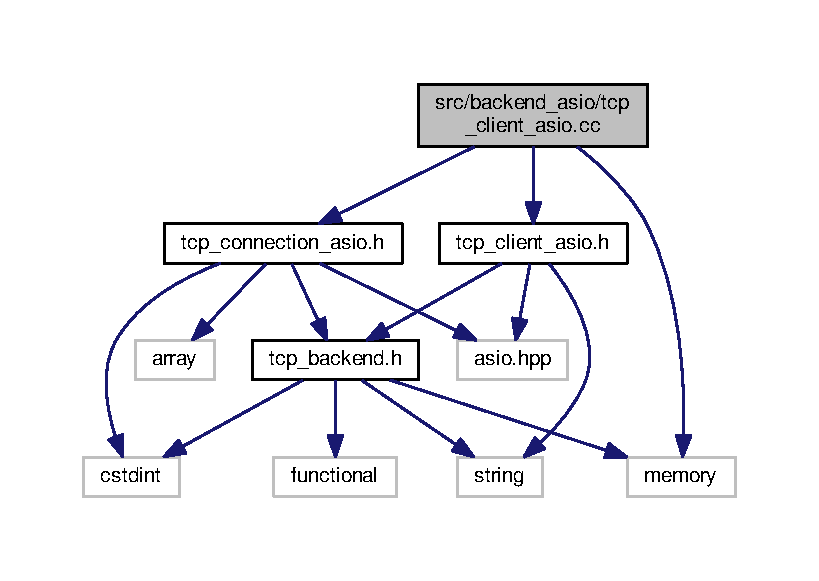
\includegraphics[width=350pt]{tcp__client__asio_8cc__incl}
\end{center}
\end{figure}
\subsection*{Namespaces}
\begin{DoxyCompactItemize}
\item 
 \hyperlink{namespaceTcpBackend}{Tcp\+Backend}
\end{DoxyCompactItemize}
\subsection*{Typedefs}
\begin{DoxyCompactItemize}
\item 
using \hyperlink{namespaceTcpBackend_a2c4e5e89eff1cb2603e717e037161b9b}{Tcp\+Backend\+::\+T\+CP} = asio\+::ip\+::tcp
\end{DoxyCompactItemize}

\hypertarget{tcp__client__asio_8h}{}\section{src/backend\+\_\+asio/tcp\+\_\+client\+\_\+asio.h File Reference}
\label{tcp__client__asio_8h}\index{src/backend\+\_\+asio/tcp\+\_\+client\+\_\+asio.\+h@{src/backend\+\_\+asio/tcp\+\_\+client\+\_\+asio.\+h}}
{\ttfamily \#include \char`\"{}tcp\+\_\+backend.\+h\char`\"{}}\newline
{\ttfamily \#include $<$string$>$}\newline
{\ttfamily \#include $<$asio.\+hpp$>$}\newline
Include dependency graph for tcp\+\_\+client\+\_\+asio.\+h\+:
\nopagebreak
\begin{figure}[H]
\begin{center}
\leavevmode
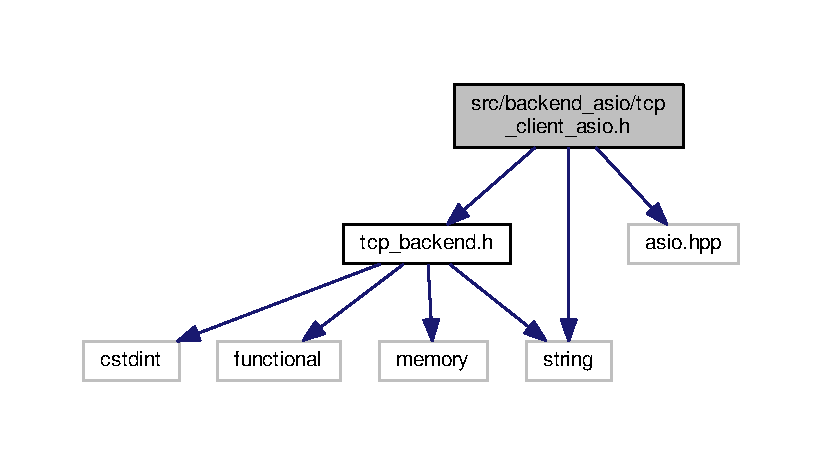
\includegraphics[width=350pt]{tcp__client__asio_8h__incl}
\end{center}
\end{figure}
This graph shows which files directly or indirectly include this file\+:
\nopagebreak
\begin{figure}[H]
\begin{center}
\leavevmode
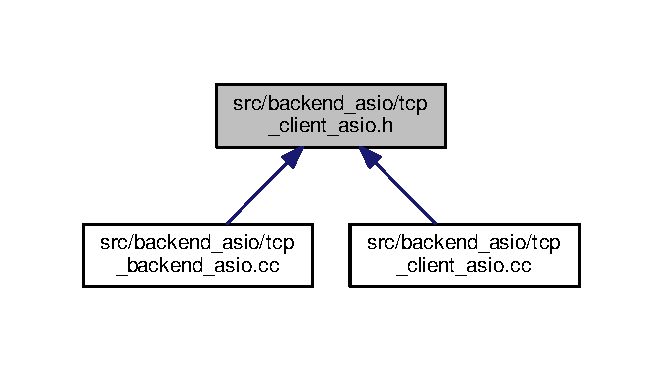
\includegraphics[width=318pt]{tcp__client__asio_8h__dep__incl}
\end{center}
\end{figure}
\subsection*{Data Structures}
\begin{DoxyCompactItemize}
\item 
class \hyperlink{classTcpBackend_1_1ClientAsio}{Tcp\+Backend\+::\+Client\+Asio}
\end{DoxyCompactItemize}
\subsection*{Namespaces}
\begin{DoxyCompactItemize}
\item 
 \hyperlink{namespaceTcpBackend}{Tcp\+Backend}
\end{DoxyCompactItemize}

\hypertarget{tcp__connection__asio_8cc}{}\section{src/backend\+\_\+asio/tcp\+\_\+connection\+\_\+asio.cc File Reference}
\label{tcp__connection__asio_8cc}\index{src/backend\+\_\+asio/tcp\+\_\+connection\+\_\+asio.\+cc@{src/backend\+\_\+asio/tcp\+\_\+connection\+\_\+asio.\+cc}}
{\ttfamily \#include \char`\"{}tcp\+\_\+connection\+\_\+asio.\+h\char`\"{}}\newline
{\ttfamily \#include $<$cstdio$>$}\newline
Include dependency graph for tcp\+\_\+connection\+\_\+asio.\+cc\+:
\nopagebreak
\begin{figure}[H]
\begin{center}
\leavevmode
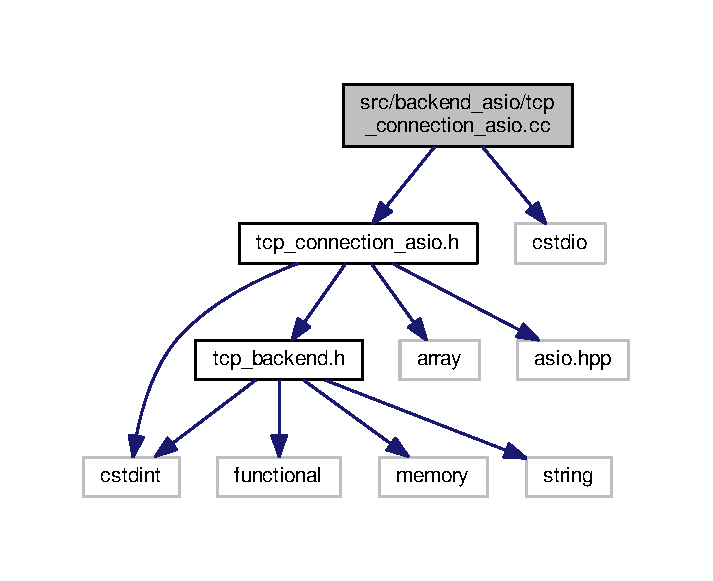
\includegraphics[width=342pt]{tcp__connection__asio_8cc__incl}
\end{center}
\end{figure}
\subsection*{Namespaces}
\begin{DoxyCompactItemize}
\item 
 \hyperlink{namespaceTcpBackend}{Tcp\+Backend}
\end{DoxyCompactItemize}

\hypertarget{tcp__connection__asio_8h}{}\section{src/backend\+\_\+asio/tcp\+\_\+connection\+\_\+asio.h File Reference}
\label{tcp__connection__asio_8h}\index{src/backend\+\_\+asio/tcp\+\_\+connection\+\_\+asio.\+h@{src/backend\+\_\+asio/tcp\+\_\+connection\+\_\+asio.\+h}}
{\ttfamily \#include \char`\"{}tcp\+\_\+backend.\+h\char`\"{}}\newline
{\ttfamily \#include $<$cstdint$>$}\newline
{\ttfamily \#include $<$array$>$}\newline
{\ttfamily \#include $<$asio.\+hpp$>$}\newline
Include dependency graph for tcp\+\_\+connection\+\_\+asio.\+h\+:
\nopagebreak
\begin{figure}[H]
\begin{center}
\leavevmode
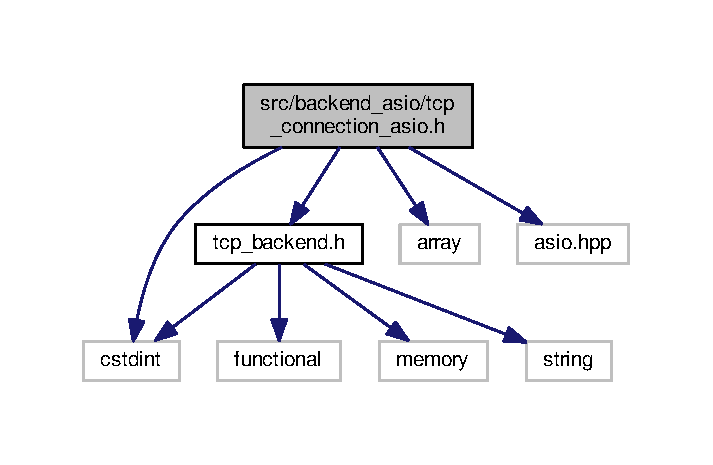
\includegraphics[width=342pt]{tcp__connection__asio_8h__incl}
\end{center}
\end{figure}
This graph shows which files directly or indirectly include this file\+:
\nopagebreak
\begin{figure}[H]
\begin{center}
\leavevmode
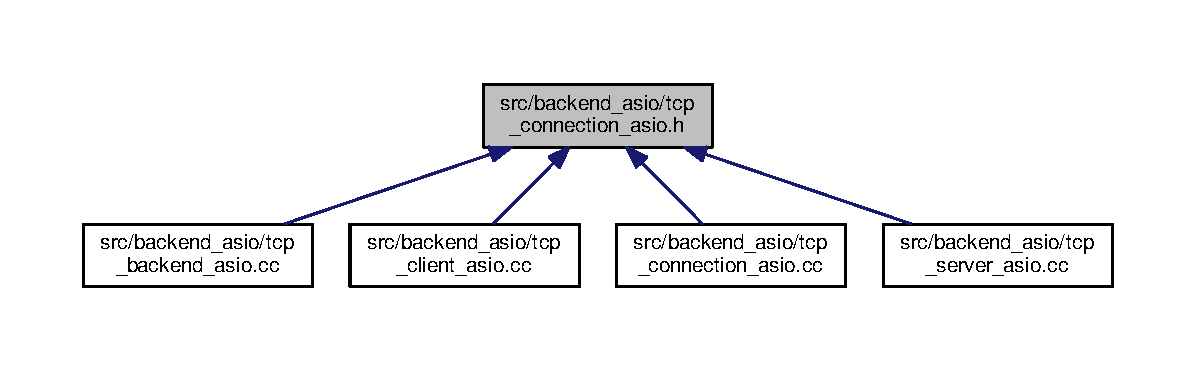
\includegraphics[width=350pt]{tcp__connection__asio_8h__dep__incl}
\end{center}
\end{figure}
\subsection*{Data Structures}
\begin{DoxyCompactItemize}
\item 
class \hyperlink{classTcpBackend_1_1ConnectionAsio}{Tcp\+Backend\+::\+Connection\+Asio}
\end{DoxyCompactItemize}
\subsection*{Namespaces}
\begin{DoxyCompactItemize}
\item 
 \hyperlink{namespaceTcpBackend}{Tcp\+Backend}
\end{DoxyCompactItemize}

\hypertarget{tcp__server__asio_8cc}{}\section{src/backend\+\_\+asio/tcp\+\_\+server\+\_\+asio.cc File Reference}
\label{tcp__server__asio_8cc}\index{src/backend\+\_\+asio/tcp\+\_\+server\+\_\+asio.\+cc@{src/backend\+\_\+asio/tcp\+\_\+server\+\_\+asio.\+cc}}
{\ttfamily \#include \char`\"{}tcp\+\_\+server\+\_\+asio.\+h\char`\"{}}\newline
{\ttfamily \#include \char`\"{}tcp\+\_\+connection\+\_\+asio.\+h\char`\"{}}\newline
Include dependency graph for tcp\+\_\+server\+\_\+asio.\+cc\+:
\nopagebreak
\begin{figure}[H]
\begin{center}
\leavevmode
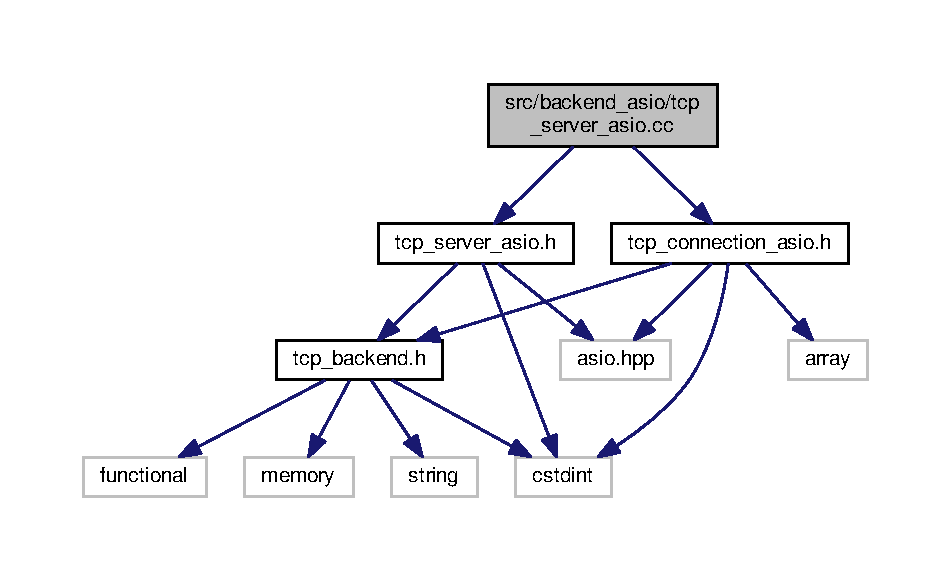
\includegraphics[width=350pt]{tcp__server__asio_8cc__incl}
\end{center}
\end{figure}
\subsection*{Namespaces}
\begin{DoxyCompactItemize}
\item 
 \hyperlink{namespaceTcpBackend}{Tcp\+Backend}
\end{DoxyCompactItemize}

\hypertarget{tcp__server__asio_8h}{}\section{src/backend\+\_\+asio/tcp\+\_\+server\+\_\+asio.h File Reference}
\label{tcp__server__asio_8h}\index{src/backend\+\_\+asio/tcp\+\_\+server\+\_\+asio.\+h@{src/backend\+\_\+asio/tcp\+\_\+server\+\_\+asio.\+h}}
{\ttfamily \#include \char`\"{}tcp\+\_\+backend.\+h\char`\"{}}\newline
{\ttfamily \#include $<$cstdint$>$}\newline
{\ttfamily \#include $<$asio.\+hpp$>$}\newline
Include dependency graph for tcp\+\_\+server\+\_\+asio.\+h\+:
\nopagebreak
\begin{figure}[H]
\begin{center}
\leavevmode
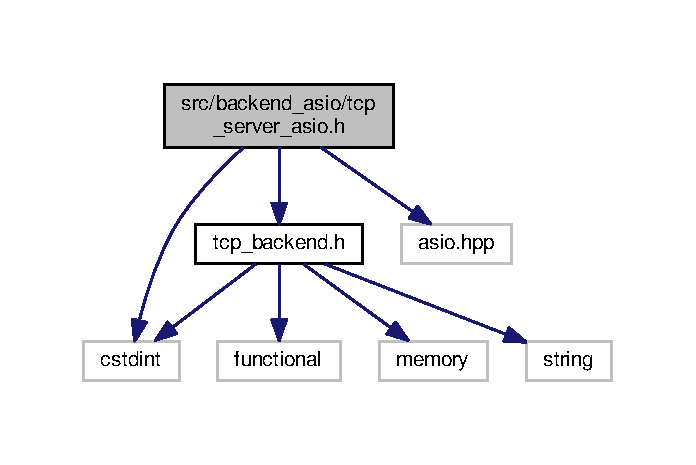
\includegraphics[width=334pt]{tcp__server__asio_8h__incl}
\end{center}
\end{figure}
This graph shows which files directly or indirectly include this file\+:
\nopagebreak
\begin{figure}[H]
\begin{center}
\leavevmode
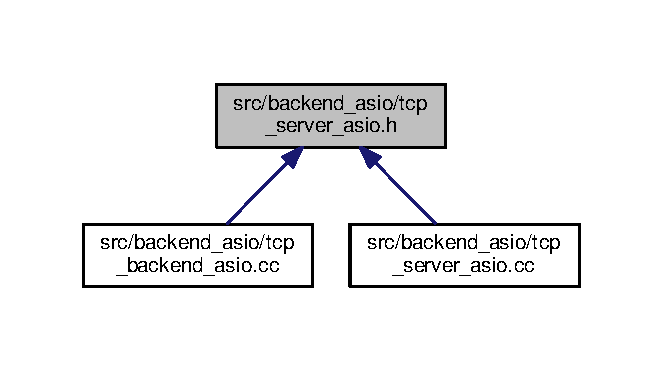
\includegraphics[width=318pt]{tcp__server__asio_8h__dep__incl}
\end{center}
\end{figure}
\subsection*{Data Structures}
\begin{DoxyCompactItemize}
\item 
class \hyperlink{classTcpBackend_1_1ServerAsio}{Tcp\+Backend\+::\+Server\+Asio}
\end{DoxyCompactItemize}
\subsection*{Namespaces}
\begin{DoxyCompactItemize}
\item 
 \hyperlink{namespaceTcpBackend}{Tcp\+Backend}
\end{DoxyCompactItemize}

\hypertarget{tcp__connection__epoll_8cc}{}\section{src/backend\+\_\+epoll/tcp\+\_\+connection\+\_\+epoll.cc File Reference}
\label{tcp__connection__epoll_8cc}\index{src/backend\+\_\+epoll/tcp\+\_\+connection\+\_\+epoll.\+cc@{src/backend\+\_\+epoll/tcp\+\_\+connection\+\_\+epoll.\+cc}}
{\ttfamily \#include \char`\"{}tcp\+\_\+connection\+\_\+epoll.\+h\char`\"{}}\newline
{\ttfamily \#include $<$unistd.\+h$>$}\newline
Include dependency graph for tcp\+\_\+connection\+\_\+epoll.\+cc\+:
\nopagebreak
\begin{figure}[H]
\begin{center}
\leavevmode
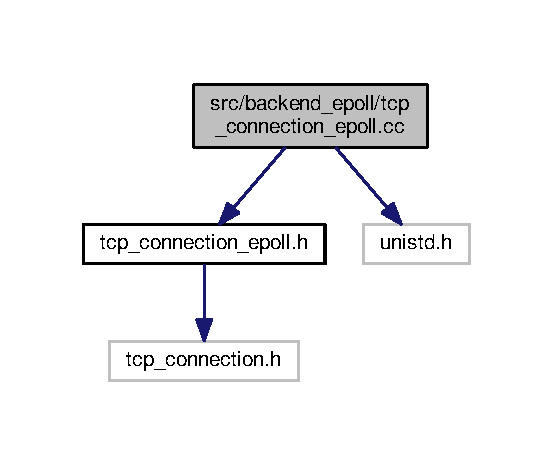
\includegraphics[width=266pt]{tcp__connection__epoll_8cc__incl}
\end{center}
\end{figure}

\hypertarget{tcp__connection__epoll_8h}{}\section{src/backend\+\_\+epoll/tcp\+\_\+connection\+\_\+epoll.h File Reference}
\label{tcp__connection__epoll_8h}\index{src/backend\+\_\+epoll/tcp\+\_\+connection\+\_\+epoll.\+h@{src/backend\+\_\+epoll/tcp\+\_\+connection\+\_\+epoll.\+h}}
{\ttfamily \#include \char`\"{}tcp\+\_\+connection.\+h\char`\"{}}\newline
Include dependency graph for tcp\+\_\+connection\+\_\+epoll.\+h\+:
\nopagebreak
\begin{figure}[H]
\begin{center}
\leavevmode
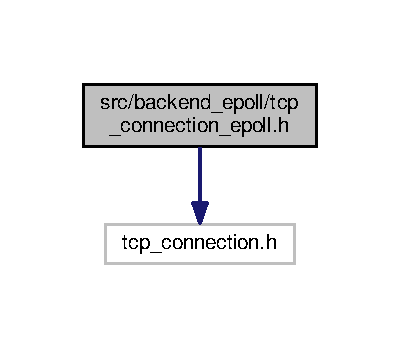
\includegraphics[width=192pt]{tcp__connection__epoll_8h__incl}
\end{center}
\end{figure}
This graph shows which files directly or indirectly include this file\+:
\nopagebreak
\begin{figure}[H]
\begin{center}
\leavevmode
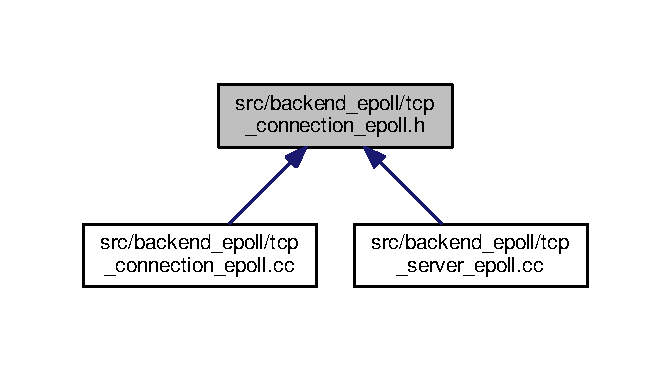
\includegraphics[width=322pt]{tcp__connection__epoll_8h__dep__incl}
\end{center}
\end{figure}
\subsection*{Data Structures}
\begin{DoxyCompactItemize}
\item 
class \hyperlink{classTcpConnectionEpoll}{Tcp\+Connection\+Epoll}
\end{DoxyCompactItemize}

\hypertarget{tcp__server__epoll_8cc}{}\section{src/backend\+\_\+epoll/tcp\+\_\+server\+\_\+epoll.cc File Reference}
\label{tcp__server__epoll_8cc}\index{src/backend\+\_\+epoll/tcp\+\_\+server\+\_\+epoll.\+cc@{src/backend\+\_\+epoll/tcp\+\_\+server\+\_\+epoll.\+cc}}
{\ttfamily \#include \char`\"{}tcp\+\_\+server\+\_\+epoll.\+h\char`\"{}}\newline
{\ttfamily \#include $<$cstdio$>$}\newline
{\ttfamily \#include $<$sys/types.\+h$>$}\newline
{\ttfamily \#include $<$sys/socket.\+h$>$}\newline
{\ttfamily \#include $<$netinet/in.\+h$>$}\newline
{\ttfamily \#include \char`\"{}tcp\+\_\+connection\+\_\+epoll.\+h\char`\"{}}\newline
Include dependency graph for tcp\+\_\+server\+\_\+epoll.\+cc\+:
\nopagebreak
\begin{figure}[H]
\begin{center}
\leavevmode
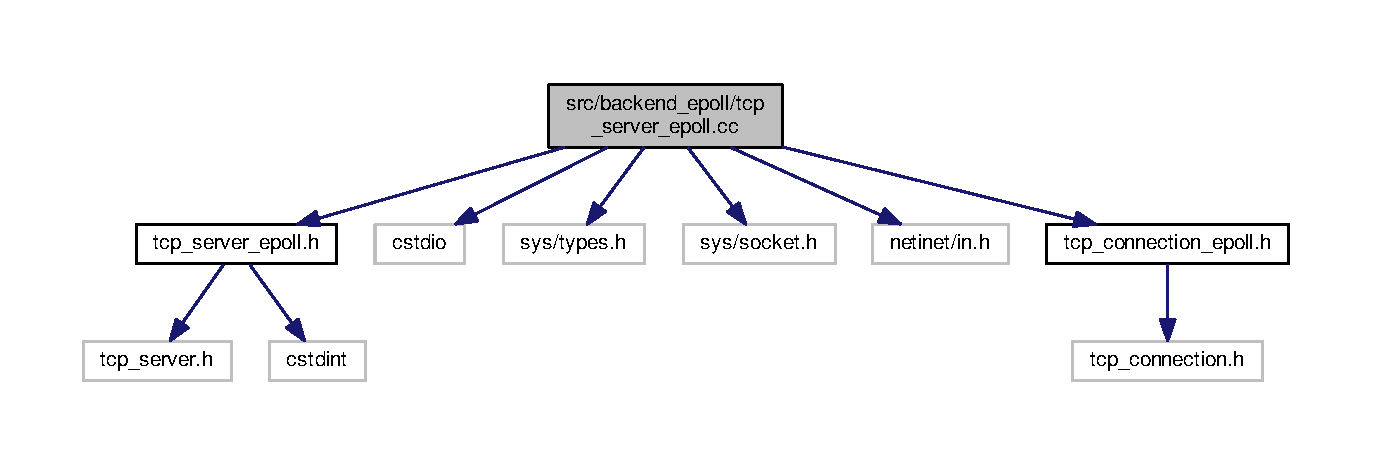
\includegraphics[width=350pt]{tcp__server__epoll_8cc__incl}
\end{center}
\end{figure}

\hypertarget{tcp__server__epoll_8h}{}\section{src/backend\+\_\+epoll/tcp\+\_\+server\+\_\+epoll.h File Reference}
\label{tcp__server__epoll_8h}\index{src/backend\+\_\+epoll/tcp\+\_\+server\+\_\+epoll.\+h@{src/backend\+\_\+epoll/tcp\+\_\+server\+\_\+epoll.\+h}}
{\ttfamily \#include \char`\"{}tcp\+\_\+server.\+h\char`\"{}}\newline
{\ttfamily \#include $<$cstdint$>$}\newline
Include dependency graph for tcp\+\_\+server\+\_\+epoll.\+h\+:
\nopagebreak
\begin{figure}[H]
\begin{center}
\leavevmode
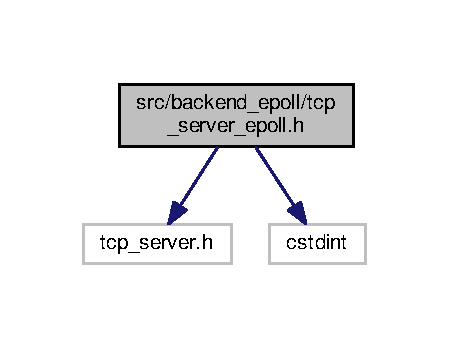
\includegraphics[width=216pt]{tcp__server__epoll_8h__incl}
\end{center}
\end{figure}
This graph shows which files directly or indirectly include this file\+:
\nopagebreak
\begin{figure}[H]
\begin{center}
\leavevmode
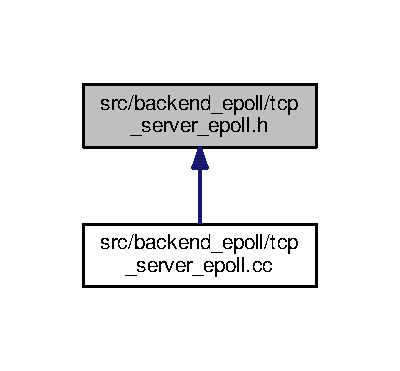
\includegraphics[width=192pt]{tcp__server__epoll_8h__dep__incl}
\end{center}
\end{figure}
\subsection*{Data Structures}
\begin{DoxyCompactItemize}
\item 
class \hyperlink{classTcpServerEpoll}{Tcp\+Server\+Epoll}
\end{DoxyCompactItemize}

\hypertarget{logger_8cc}{}\section{src/logger.cc File Reference}
\label{logger_8cc}\index{src/logger.\+cc@{src/logger.\+cc}}
{\ttfamily \#include \char`\"{}logger.\+h\char`\"{}}\newline
{\ttfamily \#include $<$cstdio$>$}\newline
{\ttfamily \#include $<$ctime$>$}\newline
{\ttfamily \#include $<$cstdarg$>$}\newline
{\ttfamily \#include $<$cstring$>$}\newline
Include dependency graph for logger.\+cc\+:
\nopagebreak
\begin{figure}[H]
\begin{center}
\leavevmode
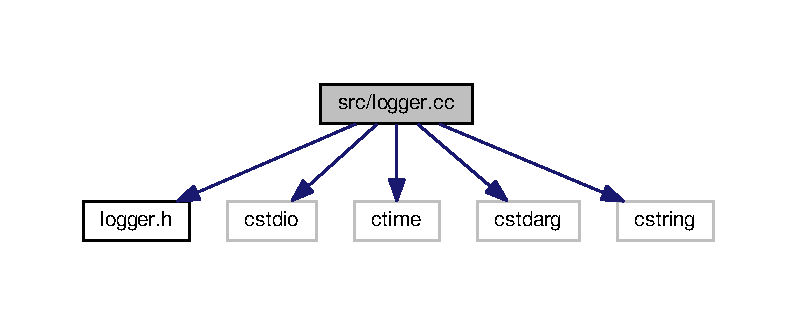
\includegraphics[width=350pt]{logger_8cc__incl}
\end{center}
\end{figure}

\hypertarget{logger_8h}{}\section{src/logger.h File Reference}
\label{logger_8h}\index{src/logger.\+h@{src/logger.\+h}}
This graph shows which files directly or indirectly include this file\+:
\nopagebreak
\begin{figure}[H]
\begin{center}
\leavevmode
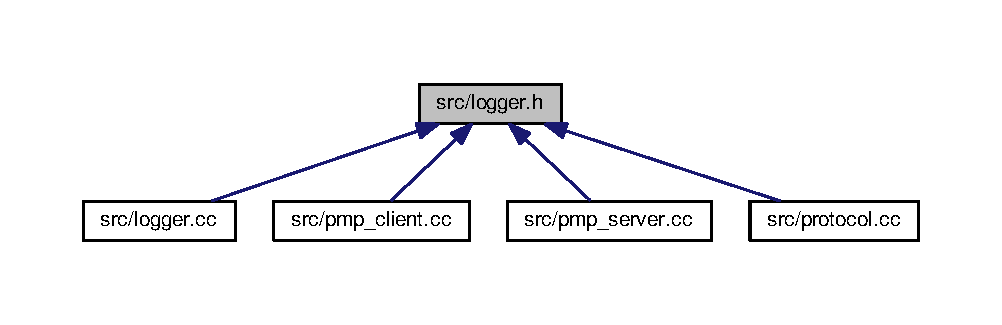
\includegraphics[width=350pt]{logger_8h__dep__incl}
\end{center}
\end{figure}
\subsection*{Namespaces}
\begin{DoxyCompactItemize}
\item 
 \hyperlink{namespaceLogger}{Logger}
\end{DoxyCompactItemize}
\subsection*{Macros}
\begin{DoxyCompactItemize}
\item 
\#define \hyperlink{logger_8h_a378e28bfcb78d17285210d6bbb70a083}{L\+O\+G\+\_\+\+I\+N\+FO}(...)~do \{ \hyperlink{namespaceLogger_a188a368bf6e884b7eba1236c39130364}{Logger\+::log}(\+\_\+\+\_\+\+F\+I\+L\+E\+\_\+\+\_\+, \+\_\+\+\_\+\+L\+I\+N\+E\+\_\+\+\_\+, \hyperlink{namespaceLogger_ad766a24576ea8b27ad9d5649cef46d8fa551b723eafd6a31d444fcb2f5920fbd3}{Logger\+::\+Level\+::\+I\+N\+FO},  \+\_\+\+\_\+\+V\+A\+\_\+\+A\+R\+G\+S\+\_\+\+\_\+); \} while(0)
\item 
\#define \hyperlink{logger_8h_a754b3d074e0af4ad3c7b918dd77ecb2d}{L\+O\+G\+\_\+\+D\+E\+B\+UG}(...)~do \{ \hyperlink{namespaceLogger_a188a368bf6e884b7eba1236c39130364}{Logger\+::log}(\+\_\+\+\_\+\+F\+I\+L\+E\+\_\+\+\_\+, \+\_\+\+\_\+\+L\+I\+N\+E\+\_\+\+\_\+, \hyperlink{namespaceLogger_ad766a24576ea8b27ad9d5649cef46d8fadc30ec20708ef7b0f641ef78b7880a15}{Logger\+::\+Level\+::\+D\+E\+B\+UG}, \+\_\+\+\_\+\+V\+A\+\_\+\+A\+R\+G\+S\+\_\+\+\_\+); \} while(0)
\item 
\#define \hyperlink{logger_8h_ad4a9117ce894e3319e903142347a0f63}{L\+O\+G\+\_\+\+E\+R\+R\+OR}(...)~do \{ \hyperlink{namespaceLogger_a188a368bf6e884b7eba1236c39130364}{Logger\+::log}(\+\_\+\+\_\+\+F\+I\+L\+E\+\_\+\+\_\+, \+\_\+\+\_\+\+L\+I\+N\+E\+\_\+\+\_\+, \hyperlink{namespaceLogger_ad766a24576ea8b27ad9d5649cef46d8fabb1ca97ec761fc37101737ba0aa2e7c5}{Logger\+::\+Level\+::\+E\+R\+R\+OR}, \+\_\+\+\_\+\+V\+A\+\_\+\+A\+R\+G\+S\+\_\+\+\_\+); \} while(0)
\end{DoxyCompactItemize}
\subsection*{Enumerations}
\begin{DoxyCompactItemize}
\item 
enum \hyperlink{namespaceLogger_ad766a24576ea8b27ad9d5649cef46d8f}{Logger\+::\+Level} \{ \hyperlink{namespaceLogger_ad766a24576ea8b27ad9d5649cef46d8fa551b723eafd6a31d444fcb2f5920fbd3}{Logger\+::\+Level\+::\+I\+N\+FO}, 
\hyperlink{namespaceLogger_ad766a24576ea8b27ad9d5649cef46d8fadc30ec20708ef7b0f641ef78b7880a15}{Logger\+::\+Level\+::\+D\+E\+B\+UG}, 
\hyperlink{namespaceLogger_ad766a24576ea8b27ad9d5649cef46d8fabb1ca97ec761fc37101737ba0aa2e7c5}{Logger\+::\+Level\+::\+E\+R\+R\+OR}
 \}
\end{DoxyCompactItemize}
\subsection*{Functions}
\begin{DoxyCompactItemize}
\item 
void \hyperlink{namespaceLogger_a188a368bf6e884b7eba1236c39130364}{Logger\+::log} (const char $\ast$filename, int line, Level level,...)
\end{DoxyCompactItemize}


\subsection{Macro Definition Documentation}
\mbox{\Hypertarget{logger_8h_a754b3d074e0af4ad3c7b918dd77ecb2d}\label{logger_8h_a754b3d074e0af4ad3c7b918dd77ecb2d}} 
\index{logger.\+h@{logger.\+h}!L\+O\+G\+\_\+\+D\+E\+B\+UG@{L\+O\+G\+\_\+\+D\+E\+B\+UG}}
\index{L\+O\+G\+\_\+\+D\+E\+B\+UG@{L\+O\+G\+\_\+\+D\+E\+B\+UG}!logger.\+h@{logger.\+h}}
\subsubsection{\texorpdfstring{L\+O\+G\+\_\+\+D\+E\+B\+UG}{LOG\_DEBUG}}
{\footnotesize\ttfamily \#define L\+O\+G\+\_\+\+D\+E\+B\+UG(\begin{DoxyParamCaption}\item[{}]{... }\end{DoxyParamCaption})~do \{ \hyperlink{namespaceLogger_a188a368bf6e884b7eba1236c39130364}{Logger\+::log}(\+\_\+\+\_\+\+F\+I\+L\+E\+\_\+\+\_\+, \+\_\+\+\_\+\+L\+I\+N\+E\+\_\+\+\_\+, \hyperlink{namespaceLogger_ad766a24576ea8b27ad9d5649cef46d8fadc30ec20708ef7b0f641ef78b7880a15}{Logger\+::\+Level\+::\+D\+E\+B\+UG}, \+\_\+\+\_\+\+V\+A\+\_\+\+A\+R\+G\+S\+\_\+\+\_\+); \} while(0)}

\mbox{\Hypertarget{logger_8h_ad4a9117ce894e3319e903142347a0f63}\label{logger_8h_ad4a9117ce894e3319e903142347a0f63}} 
\index{logger.\+h@{logger.\+h}!L\+O\+G\+\_\+\+E\+R\+R\+OR@{L\+O\+G\+\_\+\+E\+R\+R\+OR}}
\index{L\+O\+G\+\_\+\+E\+R\+R\+OR@{L\+O\+G\+\_\+\+E\+R\+R\+OR}!logger.\+h@{logger.\+h}}
\subsubsection{\texorpdfstring{L\+O\+G\+\_\+\+E\+R\+R\+OR}{LOG\_ERROR}}
{\footnotesize\ttfamily \#define L\+O\+G\+\_\+\+E\+R\+R\+OR(\begin{DoxyParamCaption}\item[{}]{... }\end{DoxyParamCaption})~do \{ \hyperlink{namespaceLogger_a188a368bf6e884b7eba1236c39130364}{Logger\+::log}(\+\_\+\+\_\+\+F\+I\+L\+E\+\_\+\+\_\+, \+\_\+\+\_\+\+L\+I\+N\+E\+\_\+\+\_\+, \hyperlink{namespaceLogger_ad766a24576ea8b27ad9d5649cef46d8fabb1ca97ec761fc37101737ba0aa2e7c5}{Logger\+::\+Level\+::\+E\+R\+R\+OR}, \+\_\+\+\_\+\+V\+A\+\_\+\+A\+R\+G\+S\+\_\+\+\_\+); \} while(0)}

\mbox{\Hypertarget{logger_8h_a378e28bfcb78d17285210d6bbb70a083}\label{logger_8h_a378e28bfcb78d17285210d6bbb70a083}} 
\index{logger.\+h@{logger.\+h}!L\+O\+G\+\_\+\+I\+N\+FO@{L\+O\+G\+\_\+\+I\+N\+FO}}
\index{L\+O\+G\+\_\+\+I\+N\+FO@{L\+O\+G\+\_\+\+I\+N\+FO}!logger.\+h@{logger.\+h}}
\subsubsection{\texorpdfstring{L\+O\+G\+\_\+\+I\+N\+FO}{LOG\_INFO}}
{\footnotesize\ttfamily \#define L\+O\+G\+\_\+\+I\+N\+FO(\begin{DoxyParamCaption}\item[{}]{... }\end{DoxyParamCaption})~do \{ \hyperlink{namespaceLogger_a188a368bf6e884b7eba1236c39130364}{Logger\+::log}(\+\_\+\+\_\+\+F\+I\+L\+E\+\_\+\+\_\+, \+\_\+\+\_\+\+L\+I\+N\+E\+\_\+\+\_\+, \hyperlink{namespaceLogger_ad766a24576ea8b27ad9d5649cef46d8fa551b723eafd6a31d444fcb2f5920fbd3}{Logger\+::\+Level\+::\+I\+N\+FO},  \+\_\+\+\_\+\+V\+A\+\_\+\+A\+R\+G\+S\+\_\+\+\_\+); \} while(0)}


\hypertarget{mandelbrot_8cc}{}\section{src/mandelbrot.cc File Reference}
\label{mandelbrot_8cc}\index{src/mandelbrot.\+cc@{src/mandelbrot.\+cc}}
{\ttfamily \#include \char`\"{}mandelbrot.\+h\char`\"{}}\newline
{\ttfamily \#include $<$cmath$>$}\newline
Include dependency graph for mandelbrot.\+cc\+:
\nopagebreak
\begin{figure}[H]
\begin{center}
\leavevmode
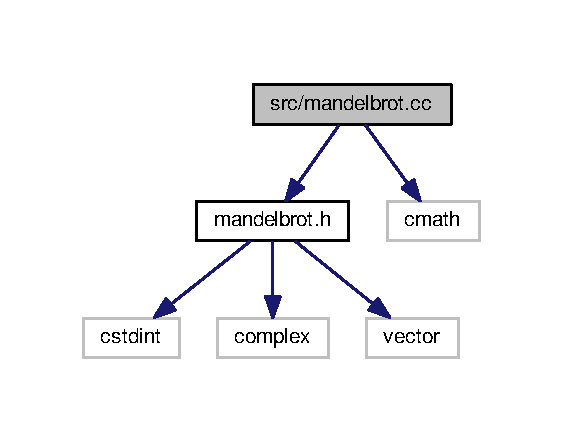
\includegraphics[width=270pt]{mandelbrot_8cc__incl}
\end{center}
\end{figure}

\hypertarget{mandelbrot_8h}{}\section{src/mandelbrot.h File Reference}
\label{mandelbrot_8h}\index{src/mandelbrot.\+h@{src/mandelbrot.\+h}}
{\ttfamily \#include $<$cstdint$>$}\newline
{\ttfamily \#include $<$complex$>$}\newline
{\ttfamily \#include $<$vector$>$}\newline
Include dependency graph for mandelbrot.\+h\+:
\nopagebreak
\begin{figure}[H]
\begin{center}
\leavevmode
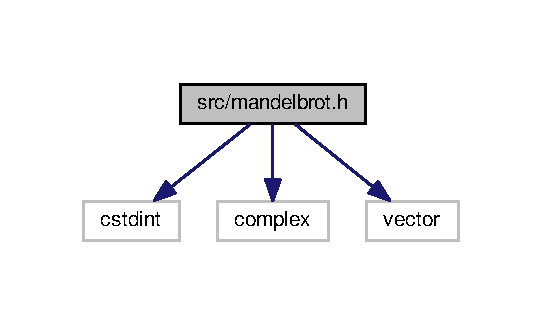
\includegraphics[width=260pt]{mandelbrot_8h__incl}
\end{center}
\end{figure}
This graph shows which files directly or indirectly include this file\+:
\nopagebreak
\begin{figure}[H]
\begin{center}
\leavevmode
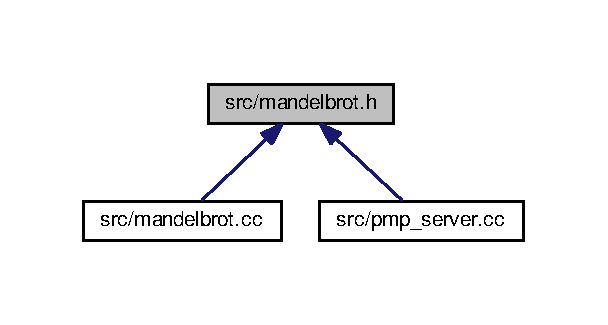
\includegraphics[width=292pt]{mandelbrot_8h__dep__incl}
\end{center}
\end{figure}
\subsection*{Namespaces}
\begin{DoxyCompactItemize}
\item 
 \hyperlink{namespaceMandelbrot}{Mandelbrot}
\end{DoxyCompactItemize}
\subsection*{Functions}
\begin{DoxyCompactItemize}
\item 
std\+::vector$<$ std\+::uint8\+\_\+t $>$ \hyperlink{namespaceMandelbrot_a232cfba00967f21fe3681d195471ef5e}{Mandelbrot\+::compute} (std\+::complex$<$ double $>$ min\+\_\+c, std\+::complex$<$ double $>$ max\+\_\+c, int image\+\_\+width, int image\+\_\+height, int max\+\_\+iter)
\begin{DoxyCompactList}\small\item\em Computes (renders) the \hyperlink{namespaceMandelbrot}{Mandelbrot} set. \end{DoxyCompactList}\end{DoxyCompactItemize}

\hypertarget{pgm_8cc}{}\section{src/pgm.cc File Reference}
\label{pgm_8cc}\index{src/pgm.\+cc@{src/pgm.\+cc}}
{\ttfamily \#include \char`\"{}pgm.\+h\char`\"{}}\newline
{\ttfamily \#include $<$fstream$>$}\newline
Include dependency graph for pgm.\+cc\+:
\nopagebreak
\begin{figure}[H]
\begin{center}
\leavevmode
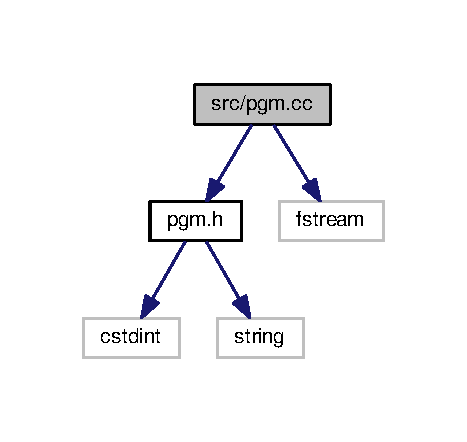
\includegraphics[width=224pt]{pgm_8cc__incl}
\end{center}
\end{figure}

\hypertarget{pgm_8h}{}\section{src/pgm.h File Reference}
\label{pgm_8h}\index{src/pgm.\+h@{src/pgm.\+h}}
{\ttfamily \#include $<$cstdint$>$}\newline
{\ttfamily \#include $<$string$>$}\newline
Include dependency graph for pgm.\+h\+:
\nopagebreak
\begin{figure}[H]
\begin{center}
\leavevmode
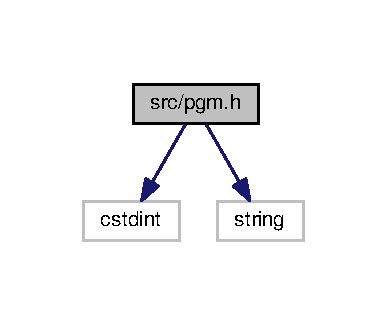
\includegraphics[width=186pt]{pgm_8h__incl}
\end{center}
\end{figure}
This graph shows which files directly or indirectly include this file\+:
\nopagebreak
\begin{figure}[H]
\begin{center}
\leavevmode
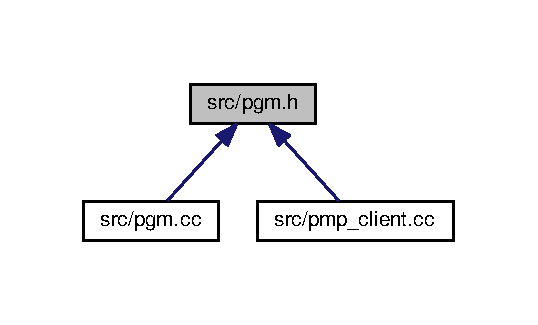
\includegraphics[width=258pt]{pgm_8h__dep__incl}
\end{center}
\end{figure}
\subsection*{Namespaces}
\begin{DoxyCompactItemize}
\item 
 \hyperlink{namespacePGM}{P\+GM}
\end{DoxyCompactItemize}
\subsection*{Functions}
\begin{DoxyCompactItemize}
\item 
void \hyperlink{namespacePGM_a564c7c26fc5370a7b3486c5ec2dec6ed}{P\+G\+M\+::write\+\_\+pgm} (const std\+::string \&filename, int width, int height, const std\+::uint8\+\_\+t $\ast$pixels)
\begin{DoxyCompactList}\small\item\em Writes a \hyperlink{namespacePGM}{P\+GM} file with the given arguments. \end{DoxyCompactList}\end{DoxyCompactItemize}

\hypertarget{pmp__client_8cc}{}\section{src/pmp\+\_\+client.cc File Reference}
\label{pmp__client_8cc}\index{src/pmp\+\_\+client.\+cc@{src/pmp\+\_\+client.\+cc}}
{\ttfamily \#include $<$cstdio$>$}\newline
{\ttfamily \#include $<$cmath$>$}\newline
{\ttfamily \#include $<$chrono$>$}\newline
{\ttfamily \#include $<$complex$>$}\newline
{\ttfamily \#include $<$deque$>$}\newline
{\ttfamily \#include $<$string$>$}\newline
{\ttfamily \#include $<$memory$>$}\newline
{\ttfamily \#include $<$vector$>$}\newline
{\ttfamily \#include $<$unordered\+\_\+map$>$}\newline
{\ttfamily \#include \char`\"{}tcp\+\_\+backend.\+h\char`\"{}}\newline
{\ttfamily \#include \char`\"{}protocol.\+h\char`\"{}}\newline
{\ttfamily \#include \char`\"{}pgm.\+h\char`\"{}}\newline
{\ttfamily \#include \char`\"{}logger.\+h\char`\"{}}\newline
Include dependency graph for pmp\+\_\+client.\+cc\+:
\nopagebreak
\begin{figure}[H]
\begin{center}
\leavevmode
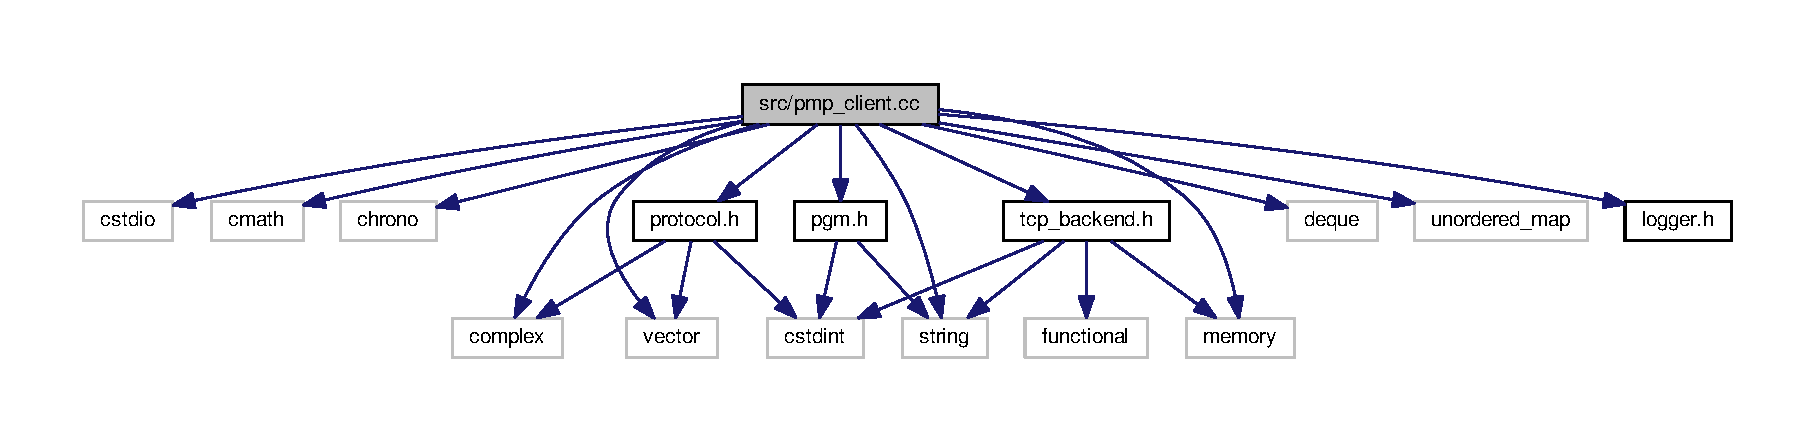
\includegraphics[width=350pt]{pmp__client_8cc__incl}
\end{center}
\end{figure}
\subsection*{Data Structures}
\begin{DoxyCompactItemize}
\item 
struct {\bfseries Arguments}
\item 
struct \hyperlink{structSession}{Session}
\end{DoxyCompactItemize}
\subsection*{Functions}
\begin{DoxyCompactItemize}
\item 
int \hyperlink{pmp__client_8cc_a0ddf1224851353fc92bfbff6f499fa97}{main} (int argc, char $\ast$argv\mbox{[}$\,$\mbox{]})
\begin{DoxyCompactList}\small\item\em Main. \end{DoxyCompactList}\end{DoxyCompactItemize}


\subsection{Function Documentation}
\mbox{\Hypertarget{pmp__client_8cc_a0ddf1224851353fc92bfbff6f499fa97}\label{pmp__client_8cc_a0ddf1224851353fc92bfbff6f499fa97}} 
\index{pmp\+\_\+client.\+cc@{pmp\+\_\+client.\+cc}!main@{main}}
\index{main@{main}!pmp\+\_\+client.\+cc@{pmp\+\_\+client.\+cc}}
\subsubsection{\texorpdfstring{main()}{main()}}
{\footnotesize\ttfamily int main (\begin{DoxyParamCaption}\item[{int}]{argc,  }\item[{char $\ast$}]{argv\mbox{[}$\,$\mbox{]} }\end{DoxyParamCaption})}



Main. 

Parses arguments. Creates Requests. Creates and starts Clients. Prints timing information.


\begin{DoxyParams}[1]{Parameters}
\mbox{\tt in}  & {\em argc} & argc \\
\hline
\mbox{\tt in}  & {\em argv} & argv\\
\hline
\end{DoxyParams}
\begin{DoxyReturn}{Returns}
exit code 
\end{DoxyReturn}

\hypertarget{pmp__server_8cc}{}\section{src/pmp\+\_\+server.cc File Reference}
\label{pmp__server_8cc}\index{src/pmp\+\_\+server.\+cc@{src/pmp\+\_\+server.\+cc}}
{\ttfamily \#include $<$cstdlib$>$}\newline
{\ttfamily \#include $<$cstdio$>$}\newline
{\ttfamily \#include $<$cstring$>$}\newline
{\ttfamily \#include $<$chrono$>$}\newline
{\ttfamily \#include $<$complex$>$}\newline
{\ttfamily \#include $<$string$>$}\newline
{\ttfamily \#include $<$unordered\+\_\+map$>$}\newline
{\ttfamily \#include $<$unistd.\+h$>$}\newline
{\ttfamily \#include \char`\"{}tcp\+\_\+backend.\+h\char`\"{}}\newline
{\ttfamily \#include \char`\"{}protocol.\+h\char`\"{}}\newline
{\ttfamily \#include \char`\"{}mandelbrot.\+h\char`\"{}}\newline
{\ttfamily \#include \char`\"{}logger.\+h\char`\"{}}\newline
Include dependency graph for pmp\+\_\+server.\+cc\+:
\nopagebreak
\begin{figure}[H]
\begin{center}
\leavevmode
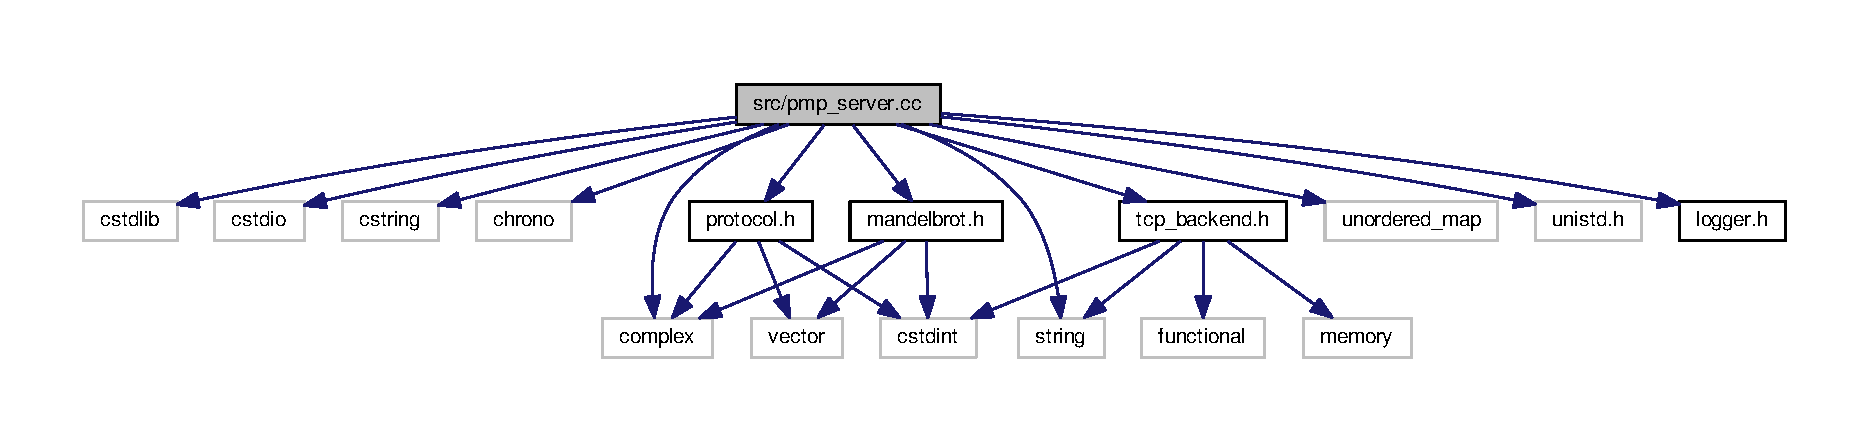
\includegraphics[width=350pt]{pmp__server_8cc__incl}
\end{center}
\end{figure}
\subsection*{Functions}
\begin{DoxyCompactItemize}
\item 
int \hyperlink{pmp__server_8cc_a0ddf1224851353fc92bfbff6f499fa97}{main} (int argc, char $\ast$argv\mbox{[}$\,$\mbox{]})
\begin{DoxyCompactList}\small\item\em Main. \end{DoxyCompactList}\end{DoxyCompactItemize}


\subsection{Function Documentation}
\mbox{\Hypertarget{pmp__server_8cc_a0ddf1224851353fc92bfbff6f499fa97}\label{pmp__server_8cc_a0ddf1224851353fc92bfbff6f499fa97}} 
\index{pmp\+\_\+server.\+cc@{pmp\+\_\+server.\+cc}!main@{main}}
\index{main@{main}!pmp\+\_\+server.\+cc@{pmp\+\_\+server.\+cc}}
\subsubsection{\texorpdfstring{main()}{main()}}
{\footnotesize\ttfamily int main (\begin{DoxyParamCaption}\item[{int}]{argc,  }\item[{char $\ast$}]{argv\mbox{[}$\,$\mbox{]} }\end{DoxyParamCaption})}



Main. 

Parses arguments. Creates and starts Server. Runs forever.


\begin{DoxyParams}[1]{Parameters}
\mbox{\tt in}  & {\em argc} & argc \\
\hline
\mbox{\tt in}  & {\em argv} & argv\\
\hline
\end{DoxyParams}
\begin{DoxyReturn}{Returns}
exit code 
\end{DoxyReturn}

\hypertarget{protocol_8cc}{}\section{src/protocol.cc File Reference}
\label{protocol_8cc}\index{src/protocol.\+cc@{src/protocol.\+cc}}
{\ttfamily \#include \char`\"{}protocol.\+h\char`\"{}}\newline
{\ttfamily \#include $<$cstdlib$>$}\newline
{\ttfamily \#include $<$iterator$>$}\newline
{\ttfamily \#include \char`\"{}logger.\+h\char`\"{}}\newline
Include dependency graph for protocol.\+cc\+:
\nopagebreak
\begin{figure}[H]
\begin{center}
\leavevmode
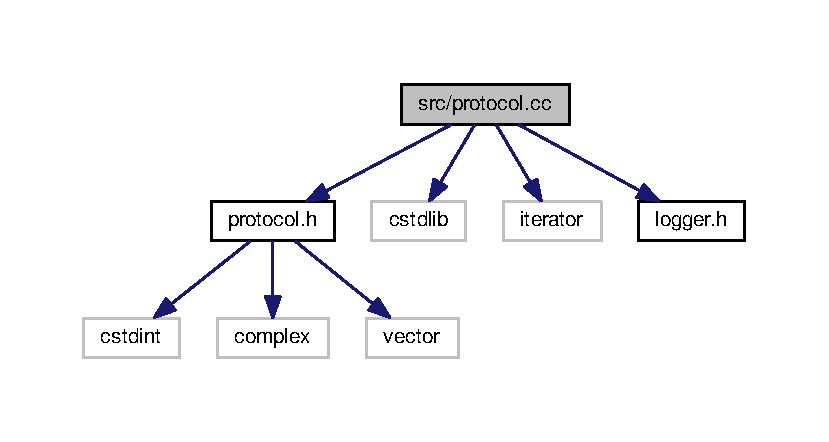
\includegraphics[width=350pt]{protocol_8cc__incl}
\end{center}
\end{figure}
\subsection*{Namespaces}
\begin{DoxyCompactItemize}
\item 
 \hyperlink{namespaceProtocol}{Protocol}
\end{DoxyCompactItemize}
\subsection*{Functions}
\begin{DoxyCompactItemize}
\item 
{\footnotesize template$<$$>$ }\\std\+::vector$<$ std\+::uint8\+\_\+t $>$ \hyperlink{namespaceProtocol_a9eadcd3ffc63dc592406a7acd8ad68bc}{Protocol\+::serialize} (const Request \&request)
\item 
{\footnotesize template$<$$>$ }\\bool \hyperlink{namespaceProtocol_a8ffab1eaeb22f833bf66d459e0779e8e}{Protocol\+::deserialize} (const std\+::vector$<$ std\+::uint8\+\_\+t $>$ \&data, Request $\ast$request)
\item 
{\footnotesize template$<$$>$ }\\std\+::vector$<$ std\+::uint8\+\_\+t $>$ \hyperlink{namespaceProtocol_a235264aa75bf1d2e3c561787c2af2573}{Protocol\+::serialize} (const Response \&response)
\item 
{\footnotesize template$<$$>$ }\\bool \hyperlink{namespaceProtocol_a89a2ebe25b5f049e779e4c451712a4d4}{Protocol\+::deserialize} (const std\+::vector$<$ std\+::uint8\+\_\+t $>$ \&data, Response $\ast$response)
\end{DoxyCompactItemize}

\hypertarget{protocol_8h}{}\section{src/protocol.h File Reference}
\label{protocol_8h}\index{src/protocol.\+h@{src/protocol.\+h}}
{\ttfamily \#include $<$cstdint$>$}\newline
{\ttfamily \#include $<$complex$>$}\newline
{\ttfamily \#include $<$vector$>$}\newline
Include dependency graph for protocol.\+h\+:
\nopagebreak
\begin{figure}[H]
\begin{center}
\leavevmode
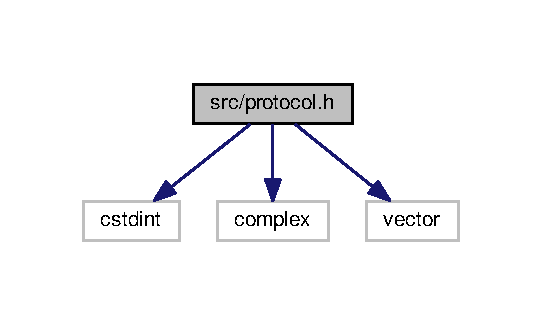
\includegraphics[width=260pt]{protocol_8h__incl}
\end{center}
\end{figure}
This graph shows which files directly or indirectly include this file\+:
\nopagebreak
\begin{figure}[H]
\begin{center}
\leavevmode
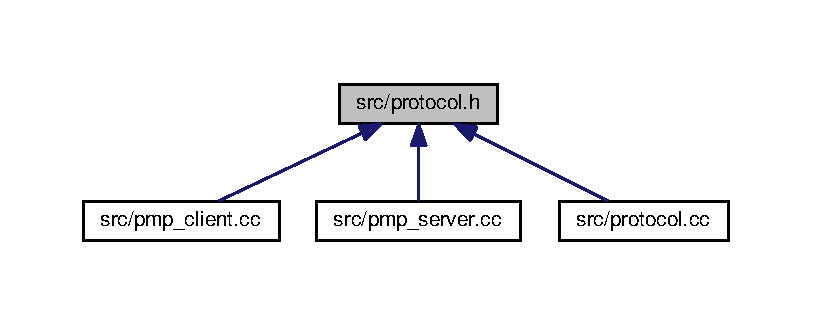
\includegraphics[width=350pt]{protocol_8h__dep__incl}
\end{center}
\end{figure}
\subsection*{Data Structures}
\begin{DoxyCompactItemize}
\item 
struct \hyperlink{structProtocol_1_1Request}{Protocol\+::\+Request}
\item 
struct \hyperlink{structProtocol_1_1Response}{Protocol\+::\+Response}
\end{DoxyCompactItemize}
\subsection*{Namespaces}
\begin{DoxyCompactItemize}
\item 
 \hyperlink{namespaceProtocol}{Protocol}
\end{DoxyCompactItemize}
\subsection*{Functions}
\begin{DoxyCompactItemize}
\item 
{\footnotesize template$<$typename T $>$ }\\std\+::vector$<$ std\+::uint8\+\_\+t $>$ \hyperlink{namespaceProtocol_aed66655af8e41eb84311b69e0f1cbbad}{Protocol\+::serialize} (const T \&message)
\item 
{\footnotesize template$<$typename T $>$ }\\bool \hyperlink{namespaceProtocol_affe27ed8631c1368f3076ccd6499fb2f}{Protocol\+::deserialize} (const std\+::vector$<$ std\+::uint8\+\_\+t $>$ \&data, T $\ast$message)
\end{DoxyCompactItemize}

\hypertarget{tcp__backend_8h}{}\section{src/tcp\+\_\+backend.h File Reference}
\label{tcp__backend_8h}\index{src/tcp\+\_\+backend.\+h@{src/tcp\+\_\+backend.\+h}}
{\ttfamily \#include $<$cstdint$>$}\newline
{\ttfamily \#include $<$functional$>$}\newline
{\ttfamily \#include $<$memory$>$}\newline
{\ttfamily \#include $<$string$>$}\newline
Include dependency graph for tcp\+\_\+backend.\+h\+:
\nopagebreak
\begin{figure}[H]
\begin{center}
\leavevmode
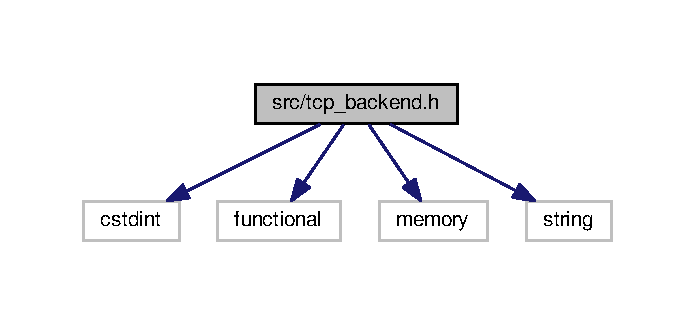
\includegraphics[width=334pt]{tcp__backend_8h__incl}
\end{center}
\end{figure}
This graph shows which files directly or indirectly include this file\+:
\nopagebreak
\begin{figure}[H]
\begin{center}
\leavevmode
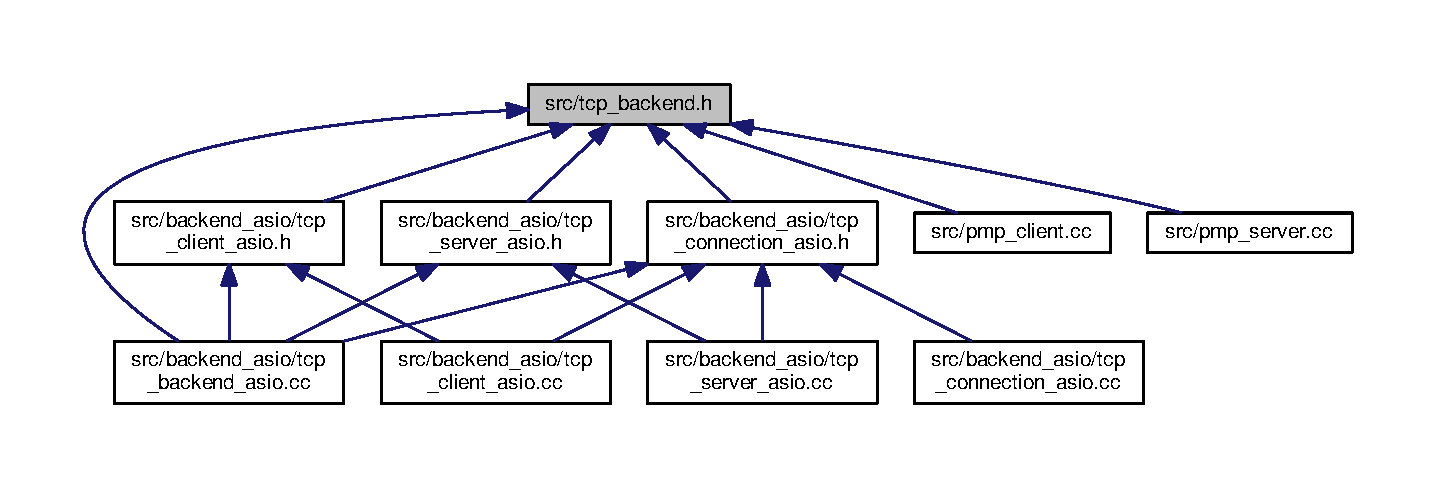
\includegraphics[width=350pt]{tcp__backend_8h__dep__incl}
\end{center}
\end{figure}
\subsection*{Data Structures}
\begin{DoxyCompactItemize}
\item 
class \hyperlink{classTcpBackend_1_1Connection}{Tcp\+Backend\+::\+Connection}
\begin{DoxyCompactList}\small\item\em Represents a connection. \end{DoxyCompactList}\item 
class \hyperlink{classTcpBackend_1_1Client}{Tcp\+Backend\+::\+Client}
\begin{DoxyCompactList}\small\item\em Used to start a connection. \end{DoxyCompactList}\item 
class \hyperlink{classTcpBackend_1_1Server}{Tcp\+Backend\+::\+Server}
\begin{DoxyCompactList}\small\item\em Used to accept new connections. \end{DoxyCompactList}\end{DoxyCompactItemize}
\subsection*{Namespaces}
\begin{DoxyCompactItemize}
\item 
 \hyperlink{namespaceTcpBackend}{Tcp\+Backend}
\end{DoxyCompactItemize}
\subsection*{Typedefs}
\begin{DoxyCompactItemize}
\item 
using \hyperlink{namespaceTcpBackend_a7d2c9f63e8017af705255d4ed08264a7}{Tcp\+Backend\+::\+On\+Read} = std\+::function$<$ void(const std\+::uint8\+\_\+t $\ast$data, int len)$>$
\begin{DoxyCompactList}\small\item\em On\+Read callback. \end{DoxyCompactList}\item 
using \hyperlink{namespaceTcpBackend_a670c71abc926680e1ea574a5f3a99135}{Tcp\+Backend\+::\+On\+Write} = std\+::function$<$ void(void)$>$
\begin{DoxyCompactList}\small\item\em On\+Write callback. \end{DoxyCompactList}\item 
using \hyperlink{namespaceTcpBackend_a17e8f044749312a6692cd0135565cbc4}{Tcp\+Backend\+::\+On\+Error} = std\+::function$<$ void(const std\+::string \&message)$>$
\begin{DoxyCompactList}\small\item\em On\+Error callback. \end{DoxyCompactList}\item 
using \hyperlink{namespaceTcpBackend_afa30fa9a706436148fb2857a2174e625}{Tcp\+Backend\+::\+On\+Connected} = std\+::function$<$ void(std\+::unique\+\_\+ptr$<$ Connection $>$ \&\&connection, const std\+::string \&address, const std\+::string \&port)$>$
\begin{DoxyCompactList}\small\item\em On\+Connected callback. \end{DoxyCompactList}\item 
using \hyperlink{namespaceTcpBackend_a2ce9b1a1f46bfa6c4b1ad38c8aa262a6}{Tcp\+Backend\+::\+On\+Disconnected} = std\+::function$<$ void(void)$>$
\begin{DoxyCompactList}\small\item\em On\+Disconnected callback. \end{DoxyCompactList}\item 
using \hyperlink{namespaceTcpBackend_a8aed04c0b1d33eb06aec746da4452484}{Tcp\+Backend\+::\+On\+Accept} = std\+::function$<$ void(std\+::unique\+\_\+ptr$<$ Connection $>$ \&\&connection)$>$
\begin{DoxyCompactList}\small\item\em On\+Accept callback. \end{DoxyCompactList}\end{DoxyCompactItemize}
\subsection*{Functions}
\begin{DoxyCompactItemize}
\item 
std\+::unique\+\_\+ptr$<$ Client $>$ \hyperlink{namespaceTcpBackend_ac561d1ab714a1b76b3db75b205dd4f84}{Tcp\+Backend\+::create\+\_\+client} (const std\+::string \&address, const std\+::string \&port, const On\+Connected \&on\+\_\+connected, const On\+Error \&on\+\_\+error)
\begin{DoxyCompactList}\small\item\em Creates a T\+CP client. \end{DoxyCompactList}\item 
std\+::unique\+\_\+ptr$<$ Server $>$ \hyperlink{namespaceTcpBackend_ad25ce62084f2e8ec8e6bd07d7510b7f2}{Tcp\+Backend\+::create\+\_\+server} (std\+::uint16\+\_\+t port, const On\+Accept \&on\+\_\+accept)
\begin{DoxyCompactList}\small\item\em Creates a T\+CP server. \end{DoxyCompactList}\item 
void \hyperlink{namespaceTcpBackend_ad949ba412696b6c7484f981fcb36a705}{Tcp\+Backend\+::run} ()
\begin{DoxyCompactList}\small\item\em Run the T\+CP backend. \end{DoxyCompactList}\end{DoxyCompactItemize}

%--- End generated contents ---

% Index
\backmatter
\newpage
\phantomsection
\clearemptydoublepage
\addcontentsline{toc}{chapter}{Index}
\printindex

\end{document}
